\chapter{局所平坦性、共変微分、曲率}

\lectureoverview{計量は、一つの選ばれた点において一次の範囲で常にユークリッド計量にすることができる。曲率は、その座標の自由度が終わるところから始まる。すなわち、隣り合う局所系が互いに整合しなくなる二次の失敗においてである。この主張を三段階で展開する。まず正規座標、次に共変微分とその接続、最後に二つの共変微分の非可換性であり、これがリーマンテンソルを定義し、潮汐重力に不変な意味を与える。}

\section{避けられない添字の重荷}

一般相対性理論は、かなり独特な仕方で難しい。その基本的な考え方は手に負えないほど難解ではないが、計算はすぐに添字、微分、記号で混み合ってくる。もっと圧縮された言語も存在する。フィールバイン、微分形式、スピノル、ツイスター、および関連する道具立ては、長い成分方程式をコンパクトな対象にまとめることができる。しかし、それらの言語を学ぶこと自体が相当な課題であり、コンパクトな記法は、最初に出会うときに最も理解する必要のある仕組みを隠してしまうことがある。

マクスウェル方程式がその手本となる。成分ごとに書けば、それらはいくつかの別々の方程式になる。ベクトル記法はそれらを発散と回転の方程式にまとめ、構造を見やすくする。一般相対性理論にも同様の圧縮が可能であるが、明示的な計算を実際に行わなければならないときには、成分による方法が依然として信頼できる道である。したがって、われわれは添字を目に見える形に保つ。その文法に慣れてしまえば、計算が依然として何ページも埋めることがあっても、概念的経路はずっと滑らかになる。

記号計算機パッケージはその計算の助けになる。計量\(g_{mn}(x)\)が与えられれば、そのようなパッケージはクリストッフェル記号、リーマンテンソル、リッチテンソル、アインシュタインテンソルを構成できる。さらにこれらの表式を場の方程式に代入できる。これは対象が何を意味するかを理解する必要を取り除くものではない。単に機械的な展開を幾何学から分離するだけである。

\begin{classroomqa}
\audiencequestion{この講義の時点で、一般相対性理論の研究の活発な領域は何であったか。}
\lecturerresponse{講義はいくつかの前線を特に取り上げた。量子重力とブラックホールの量子物理学は、基礎理論における中心的な問題であった。古典的宇宙物理学と数値相対性理論は、連星ブラックホールの周回や合体のような系を研究した。そこでは、アインシュタイン方程式を解き、重力放射を予測するには、方程式を盲目的に計算機に投入するだけではるかに及ばない。同じ数学的構造は、物性物理学や流体力学でも用いられつつあった。歴史的な点も同様に際立っていた。一般相対性理論は、1960年代には比較的小さな専門分野から、量子場の理論と密接に結びついた理論物理学の中心的な言語の一つへと移り変わったのである。
\lecturetimestamp{00:05:15}}
\end{classroomqa}

これはリーマン幾何学それ自体に充てる最後の講義である。次の講義から、その幾何学は重力として解釈される。橋はすでに見えている。加速座標系や曲線座標系に起因する見かけの場から真の重力場を区別することは、数学的には、扱いにくい座標で書かれた平坦な計量から曲がった計量を区別することと同じ問題である。

\section{不変な問い}

二次元幾何学は、ユークリッド幾何学が内在的に成り立つとき平坦である。すなわち、直線、平行線、三角形の関係、距離の測定がすべてユークリッド的な形をとる。平坦性とは
\(g_{mn}=\delta_{mn}\)
を意味すると言いたくなるが、その主張は座標に依存する。通常の平面でさえ、極座標では位置に依存する計量をもつ。正しい主張は、平坦な領域は、その領域全体で計量が定数かつユークリッド的となる座標を許す、というものである。

代わりに、計量が何らかの任意の座標で与えられたとしよう。悪い判定法の一つは、座標系を次々に探し、そのたびに計量を変換し、最終的にデカルト形式を見つけることを期待するものであろう。可能性は無限にあるので、これは実用的な判定基準ではない。

正しい戦略は、\(g_{mn}\)とその導関数から診断量を構成することである。われわれは二つの決定的な性質をもつ対象\(R\)を望む。
\[
\begin{aligned}
R=0
&\quad\Longleftrightarrow\quad
\text{locally flat geometry},\\
R\neq 0 \text{ at } P
&\quad\Longrightarrow\quad
\text{curvature at } P.
\end{aligned}
\]
最も重要なことに、\(R\)はテンソルでなければならない。一つの座標系で消えるテンソルはすべての座標系で消えるので、座標の探索は不要である。

\begin{figure}[H]
\centering
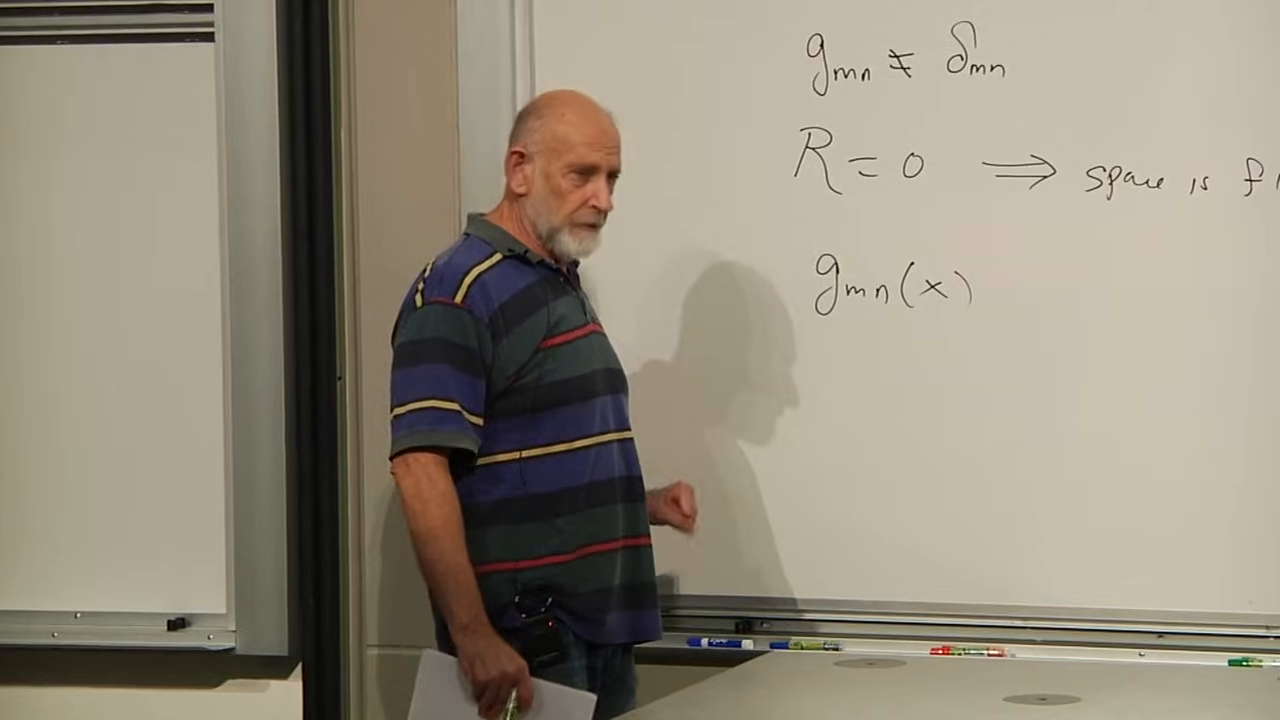
\includegraphics[width=\linewidth]{lecture_03_figure_01.png}
\caption{望ましい不変な判定法。計量は見た目上\(\delta_{mn}\)に等しい必要はないが、消える曲率対象は局所的に平坦な幾何学を同定するはずである。}
\lectureframe{00:18:20}
\end{figure}

\emph{局所的}という限定は重要である。リーマン・テンソルが消えることは局所的なユークリッド幾何を保証するが、大域的な同一視によって非自明な位相が生じることもある。例えば平坦な円筒や平坦なトーラスは、大域的に平面でなくても局所的にユークリッドでありうる。

\section{微小領域における計量幾何}

次元によって何が変わるかを見ると理解しやすい。零次元空間は一点にすぎない。連結な一次元リーマン空間は局所的に直線に伸ばすことができるが、大域的には区間、直線、またはループでありうる。閉じた一次元の軌道上に閉じ込められた虫はその周長を測ることができるが、周囲の部屋の中で軌道を曲げてもその内在的計量は変わらない。

二次元でははるかに豊かな内在的幾何が許される。平面、球面、でこぼこした地球表面、トーラスは局所的にさえ一致する必要はなく、その大域的位相も異なりうる。計量はそれらの無限小距離を記録する道具である：
\begin{equation}
 ds^2=g_{mn}(x)\,dx^m dx^n.
\label{eq:l3-line-element}
\end{equation}
量\(ds^2\)はスカラーである。したがって座標変換の下での\(dx^m\)の変化は、\(g_{mn}\)の変換によって正確に相殺される。

\begin{figure}[H]
\centering
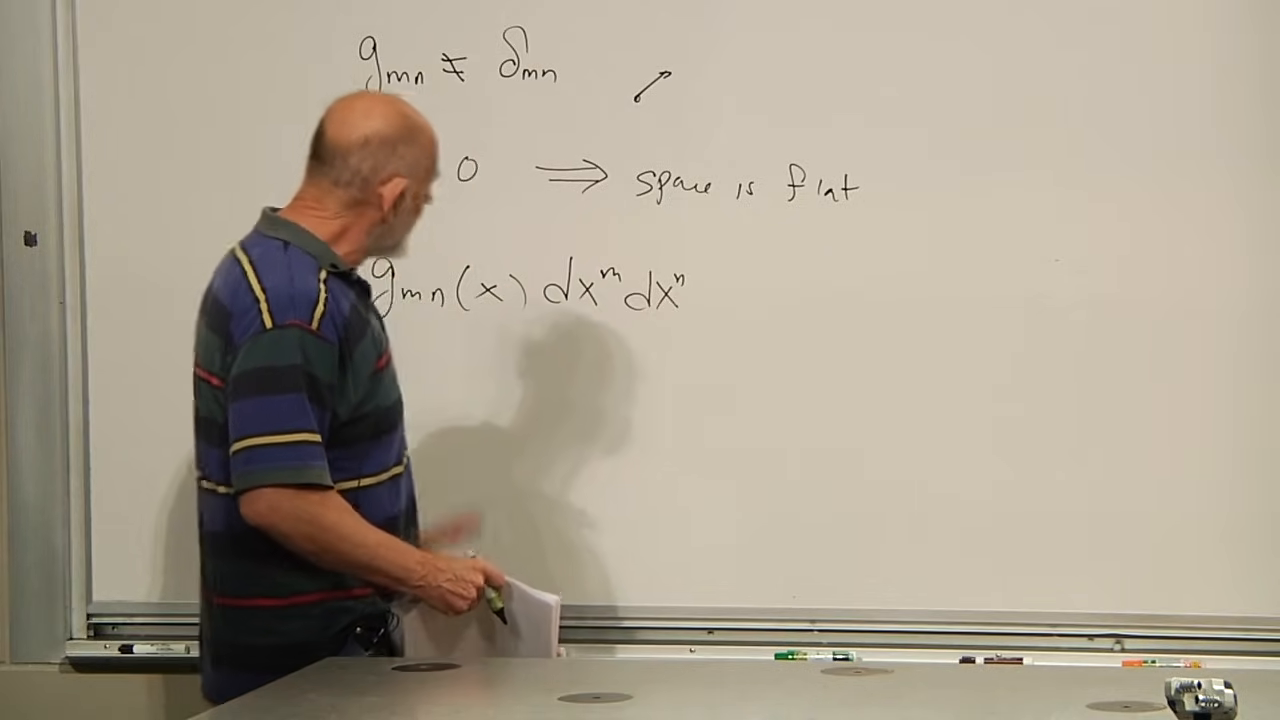
\includegraphics[width=\linewidth]{lecture_03_figure_02.png}
\caption{位置に依存する計量で書かれた不変線素。}
\lectureframe{00:19:00}
\end{figure}

計量は非退化であり、したがって逆計量をもつ：
\begin{equation}
 g^{mn}g_{nr}=\delta^m{}_r.
\label{eq:l3-inverse-metric}
\end{equation}
混合クロネッカー・テンソル\(\delta^m{}_r\)は恒等写像である。通常のリーマン幾何では計量は正定値でもある：
\begin{equation}
 g_{mn}u^m u^n>0
\qquad\text{for every nonzero }u^m.
\label{eq:l3-positive}
\end{equation}
ローレンツ時空では後にこの正定値性を緩めつつ、非退化性は保持する。

\begin{figure}[H]
\centering
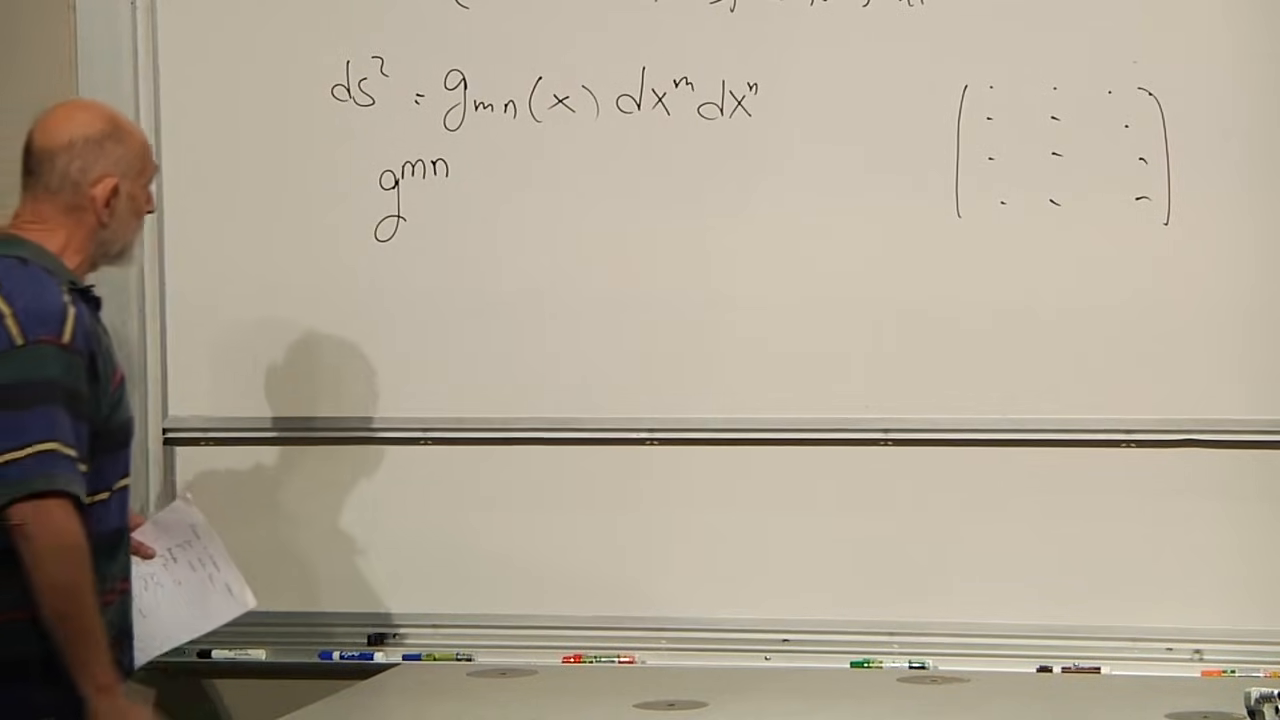
\includegraphics[width=\linewidth]{lecture_03_figure_03.png}
\caption{逆計量と恒等テンソル（黒板）。}
\lectureframe{00:20:40}
\end{figure}

計量はベクトルとコベクトルを同一視する：
\begin{equation}
 V_m=g_{mn}V^n,
 \qquad
 V^m=g^{mn}V_n.
\label{eq:l3-raise-lower}
\end{equation}
したがって添字を動かすことは計量によって行われる操作であり、活字上の変更ではない。

\begin{figure}[H]
\centering
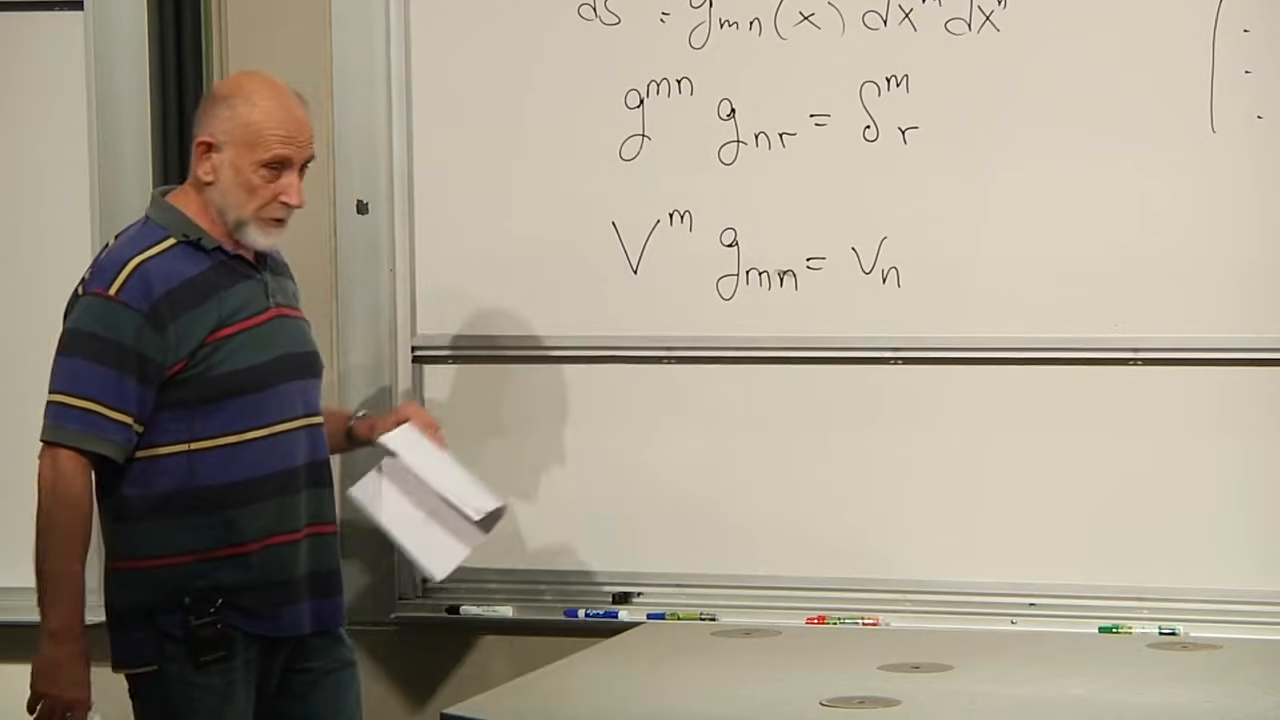
\includegraphics[width=\linewidth]{lecture_03_figure_04.png}
\caption{計量とその逆計量によるベクトルの添字の上げ下げ。}
\lectureframe{00:24:40}
\end{figure}

ある領域で\(g_{mn}\)のすべての成分が定数であれば、定数係数の線形座標変換によってそこで計量を対角化し規格化できる。そのとき幾何は平坦である。したがって興味深い情報は、計量が位置とともにどのように変化するかに結びついていなければならない。

\section{正規座標：一次まで平坦}

点\(P\)を選ぶ。正規座標定理によれば、\(P\)を中心とする座標であって
\begin{align}
 g_{mn}(P)&=\delta_{mn}, \label{eq:l3-normal-metric}\\
 \partial_r g_{mn}(P)&=0. \label{eq:l3-normal-first}
\end{align}
を満たすものを構成できる。講義ではこれをガウス正規座標と呼ぶ。幾何学的には、\(P\)を通る軸を引き、その座標線を幾何が許す限りまっすぐに延ばす。まっすぐさの正確な概念は後に測地線運動となる。

\begin{figure}[H]
\centering
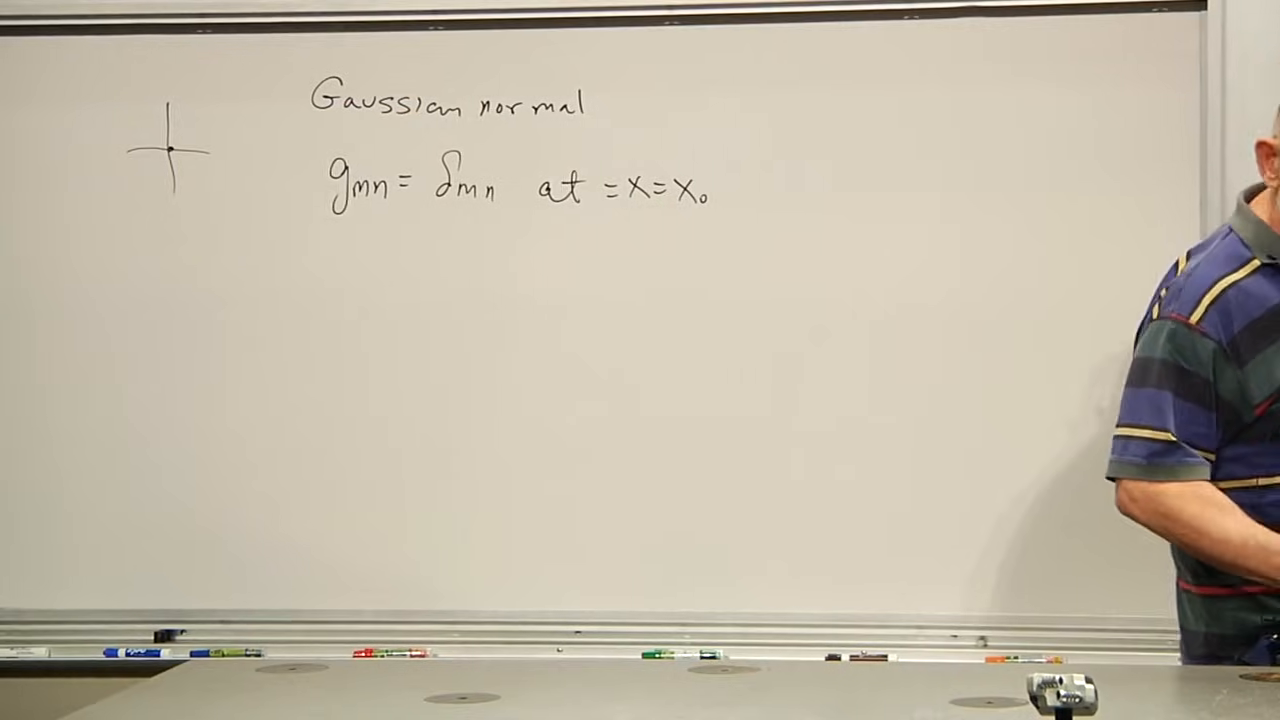
\includegraphics[width=\linewidth]{lecture_03_figure_05.png}
\caption{選んだ点で計量がユークリッドとなるように選ばれた正規座標。}
\lectureframe{00:28:50}
\end{figure}

そのような枠は一意ではない。\(P\)における直交回転は\(g_{mn}(P)=\delta_{mn}\)を保つ。重要なのは軸の向きではなく、\eqref{eq:l3-normal-metric}と\eqref{eq:l3-normal-first}の両方が成り立つ枠が存在することである。

\begin{classroomqa}
\audiencequestion{これらの条件は選んだ点でのみ成り立つのか、それとも近傍全体で成り立つのか。}
\lecturerresponse{それらは選んだ点\(P\)で成り立つ。正規枠は任意の点を中心に置くことができるが、曲がった領域にわたって単一の座標系を用い、計量をユークリッドに保ちつつすべての一次導関数を至る所で零にすることは一般にはできない。同じ座標を\(P\)から離れたところまで延ばすと、計量のより高次の導関数が現れる。
\lecturetimestamp{00:29:53}}
\end{classroomqa}

\(P\)では、二次導関数は一般に避けられない：
\begin{equation}
 \partial_r\partial_s g_{mn}(P)\neq 0
 \qquad\text{in general}.
\label{eq:l3-normal-second}
\end{equation}
したがって計量は、一点における零次または一次では不変な曲率の情報を担わない。座標の自由度がそれを除去できるからである。最初に可能な不変な情報は二次で現れる。

\begin{figure}[H]
\centering
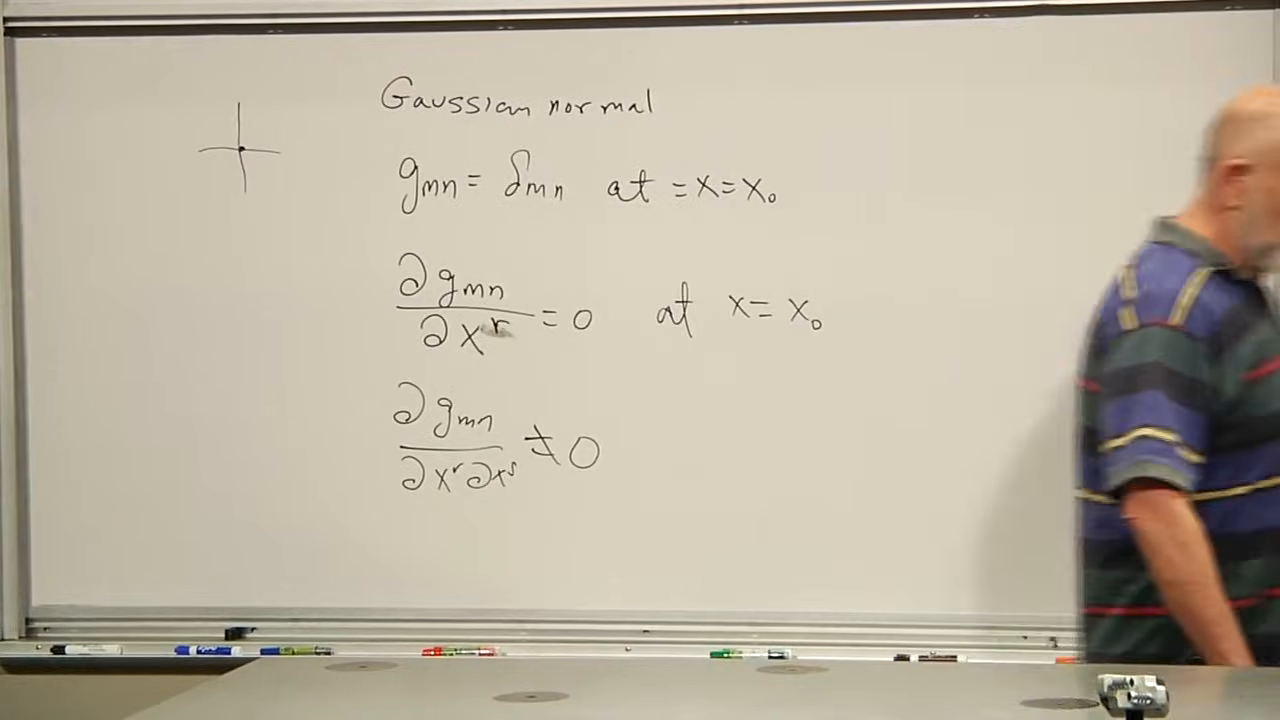
\includegraphics[width=\linewidth]{lecture_03_figure_06.png}
\caption{正規座標の条件：計量はユークリッドであり、その一次導関数は消え、二次導関数は消える必要はない。}
\lectureframe{00:30:50}
\end{figure}

\subsection{なぜ座標の自由度で十分なのか}

\(P\)を座標\(x^m\)と\(y^m\)の共通の原点とする。線形変換を用いて原点における計量を整えた後、さらなる座標変換の二次の部分を考える：
\begin{equation}
 x^m
 =y^m+C^m{}_{nr}y^n y^r+O(y^3),
 \qquad C^m{}_{nr}=C^m{}_{rn}.
\label{eq:l3-quadratic-transform}
\end{equation}
四次元では対称な対\(nr\)は
\[
\frac{4(4+1)}{2}=10
\]
個の独立な選択をもつ。\(m\)の四つの値のそれぞれについて、十個の係数\(C^m{}_{nr}\)があり、四十個の二次係数を与える。

対称計量もまた四次元では十個の独立な成分をもつ。各成分は四つの一階導関数をもつので、条件\(\partial_r g_{mn}(P)=0\)は四十個の方程式を構成する。この数の一致は、二次の座標自由度が一階導関数の条件を課すのにちょうど適切な大きさであることを示している。正規座標定理が存在の主張を与える。数え上げだけでは、任意の非線形系に対する可解性の完全な証明ではなく、有用な構造的検査にすぎない。

\begin{figure}[H]
\centering
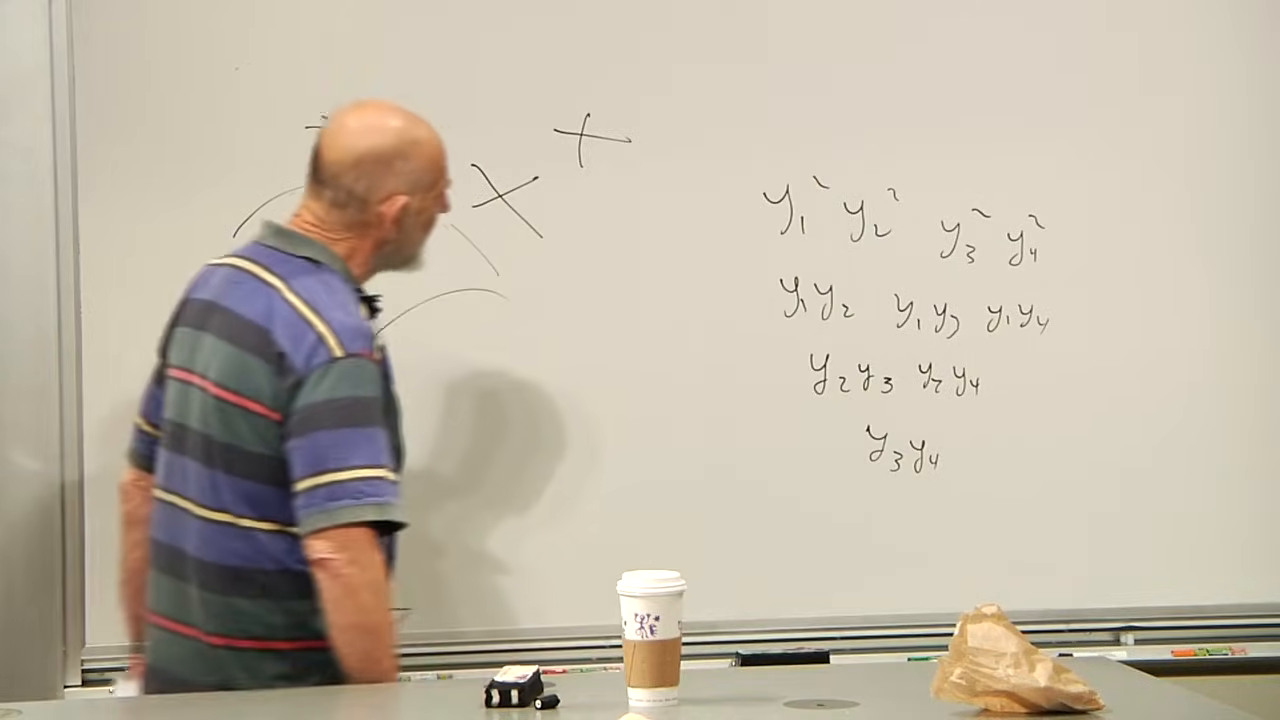
\includegraphics[width=\linewidth]{lecture_03_figure_07.png}
\caption{二次の座標変換と四次元における十個の独立な二次単項式。}
\lectureframe{00:33:50}
\end{figure}

\begin{classroomqa}
\audiencequestion{\(x^m=y^m+C^m{}_{nr}y^n y^r+\cdots\)は座標変換の試みか。}
\lecturerresponse{はい。係数\(C^m{}_{nr}\)は、新しい座標において計量の一階導関数が共通の原点で消えるように選ばれる。線形部分はその点の近くでヤコビアンを可逆に保ち、二次部分は計量の一階導関数を調整する。\lecturetimestamp{00:35:41}}
\end{classroomqa}

\begin{classroomqa}
\audiencequestion{滑らかな幾何が局所的に平坦であるというのはこのことを意味するのか。}
\lecturerresponse{それは関連する一次の主張である。十分小さなスケールでは、滑らかな曲面はその接平面で近似され、正規座標はその事実を\(g_{mn}(P)=\delta_{mn}\)と\(\partial_r g_{mn}(P)=0\)を通じて表現する。近傍における厳密な平坦性はより強く、そこでは曲率テンソルも消えることを要求する。\lecturetimestamp{00:36:19}}
\end{classroomqa}

\begin{classroomqa}
\audiencequestion{四十個の係数と四十個の方程式の一致は、本当に方程式が解けることを保証するのか。}
\lecturerresponse{数え上げは必要な座標自由度を特定し、定理は滑らかで非退化な計量に対する局所的な構成を保証する。講義では二次元の場合を直接確かめることを演習として提案している。この議論は四次元に依存しない。\(d\)次元でも同じ対称性と座標自由度が整合する。\lecturetimestamp{00:36:45}}
\end{classroomqa}

\begin{classroomqa}
\audiencequestion{なぜ展開に定数項がなく、どの項が一次なのか。}
\lecturerresponse{項\(y^m\)が一次の項である。定数項が省略されたのは、二つの座標原点が同じ点を表すように意図的に選ばれたからであり、したがって\(y=0\)は\(x=0\)を意味する。この選択は一般性を損なわない。\lecturetimestamp{00:38:52}}
\end{classroomqa}

\section{成分ごとの微分が失敗する理由}

次に共変ベクトル場\(V_m(x)\)を考える。平坦空間上の直交デカルト座標では、幾何学的に一定なベクトルは一定の成分をもつ。したがってその導関数を\(\partial_rV_m\)と定義しようと試みるかもしれない。困難は座標格子が曲がるとすぐに現れる。

\begin{figure}[H]
\centering
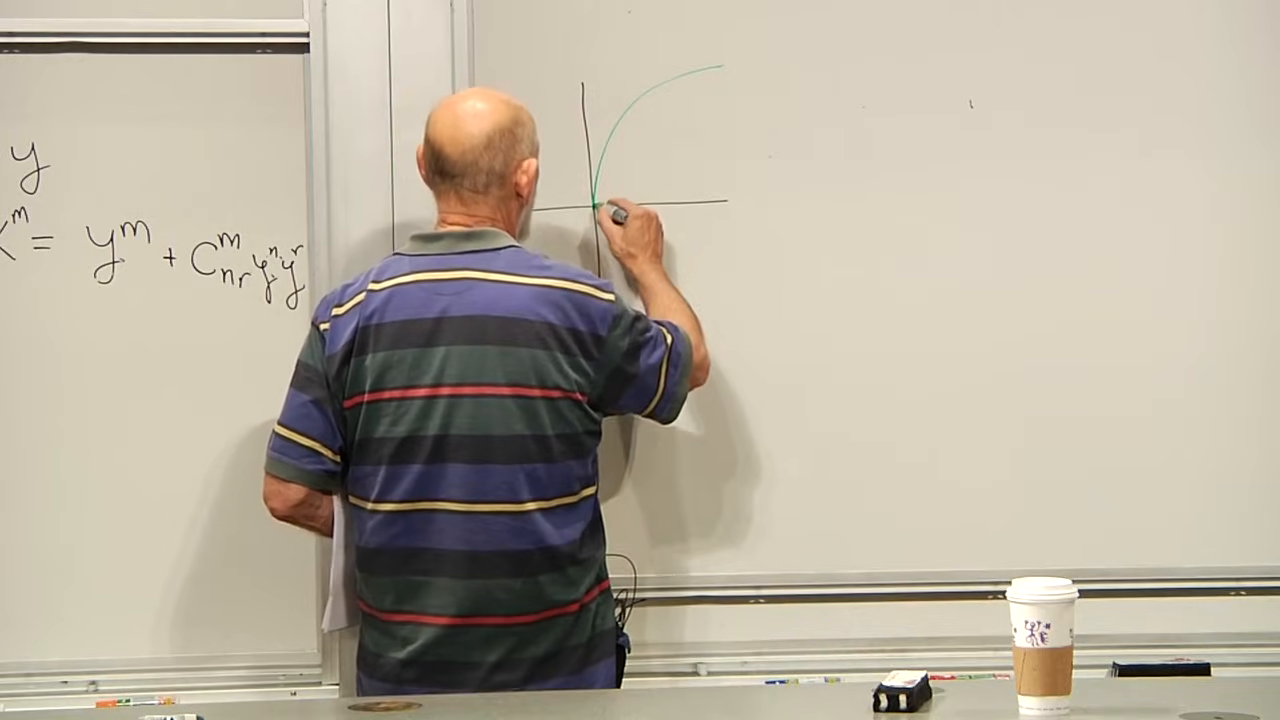
\includegraphics[width=\linewidth]{lecture_03_figure_08.png}
\caption{局所的に直線的な枠に重ねられた曲線座標格子。}
\lectureframe{00:40:10}
\end{figure}

同じ幾何学的ベクトルを隣接する点に置く。固定されたデカルト枠に対して成分は変化しない。しかし曲線基底に対しては、移動するにつれて基底ベクトル自体が回転するので、ベクトルが変化しなくても成分のリストは変化する。

\begin{figure}[H]
\centering
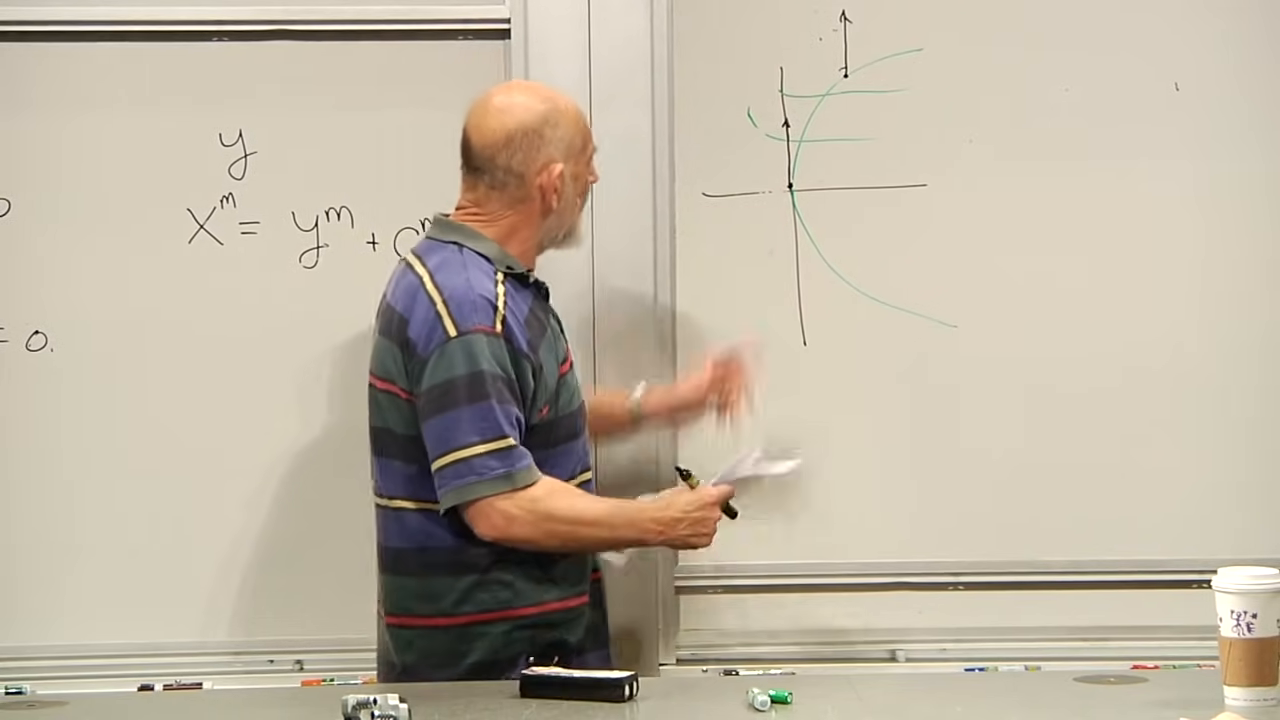
\includegraphics[width=\linewidth]{lecture_03_figure_09.png}
\caption{隣接する点における同じベクトルが、局所座標基底が回転したために異なる成分をもつ。}
\lectureframe{00:42:30}
\end{figure}

したがって素朴な条件
\begin{equation}
 \partial_rV_m=0
\label{eq:l3-naive-derivative}
\end{equation}
は、ある座標系では真であり別の座標系では偽でありうる。もし\(\partial_rV_m\)が二階のテンソルであれば、それは不可能であろう。一つの枠で消えることはすべての枠で消えることを意味するからである。したがってベクトル成分の通常の偏導関数はテンソル成分ではない。

\begin{figure}[H]
\centering
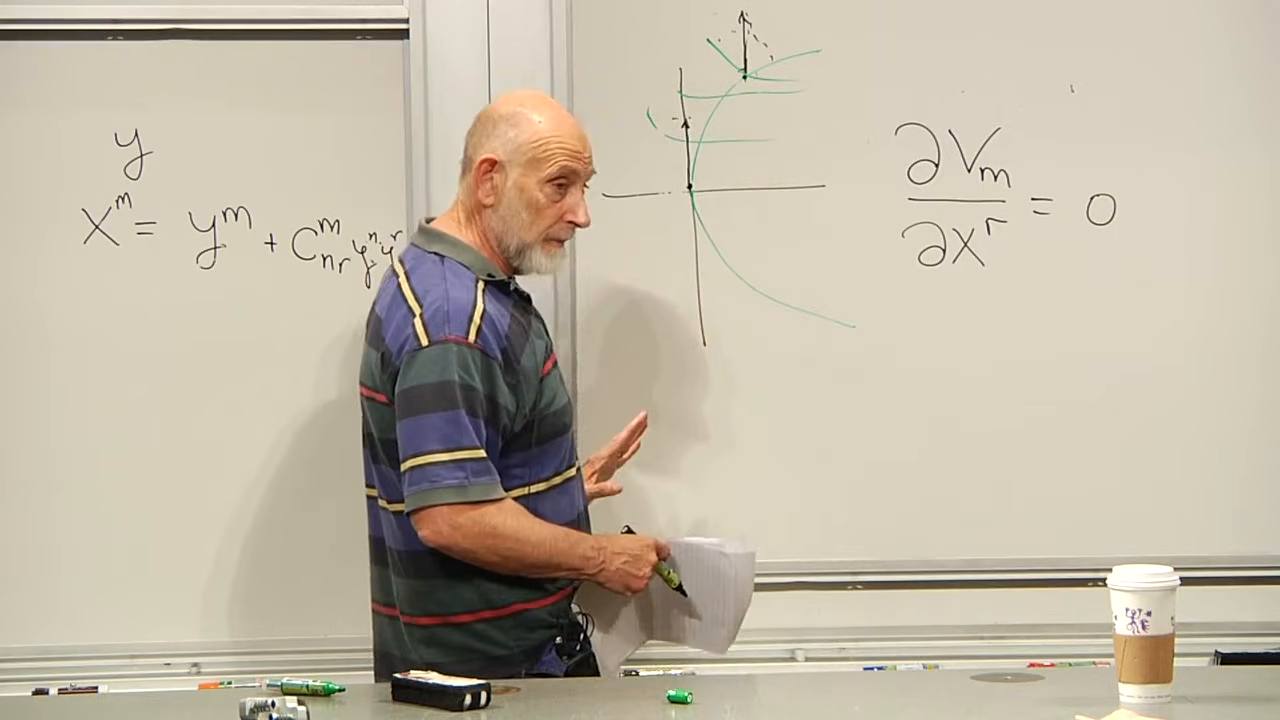
\includegraphics[width=\linewidth]{lecture_03_figure_10.png}
\caption{変化する曲線基底の隣に置かれた、意図的に素朴なゼロ導関数条件。}
\lectureframe{00:44:00}
\end{figure}

基底による見かけの変化を取り除きつつ、ベクトル場の真の変化を保持する導関数が必要である。

\section{共変導関数の定義}

\(P\)における微分は、\(P\)の任意に小さな近傍における値のみを比較する。したがってそこを中心とする正規座標で始めればよい。隣接する点のベクトルを取り、その尾を\(P\)に戻し、移動の間その正規座標成分を固定しておく。移動されたベクトルと\(P\)にすでにあるベクトルを比較し、その差を隔たりで割ると、その局所的に直線的な枠における通常の導関数が得られる。

\begin{figure}[H]
\centering
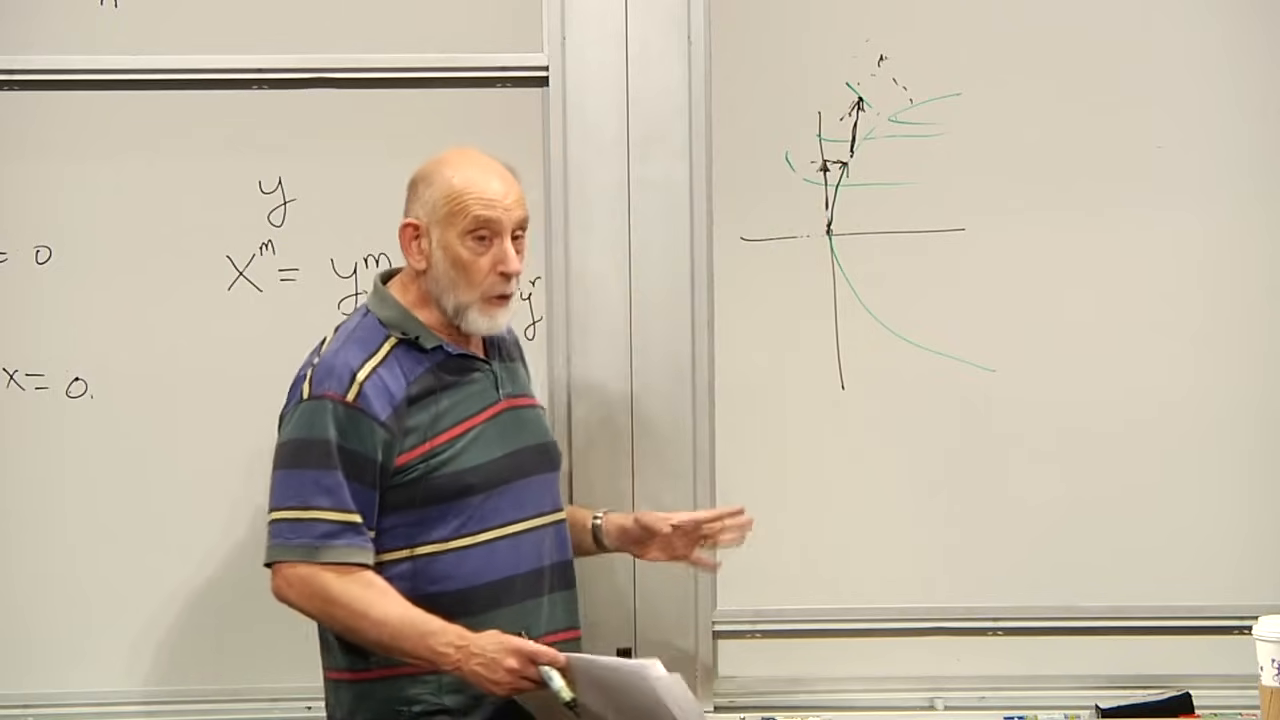
\includegraphics[width=\linewidth]{lecture_03_figure_11.png}
\caption{局所的な比較：差を取る前に隣接ベクトルを正規座標で平行移動する。}
\lectureframe{00:46:50}
\end{figure}

次に、その幾何学的に定義された微分を任意の座標で表そう。寄与は二つある。成分\(V_m\)が変化しうること、そして座標基底が変化しうることである。添字構造が補正項の形を決める：
\begin{equation}
 \nabla_rV_m
 =\partial_rV_m-\Gamma^t{}_{rm}V_t.
\label{eq:l3-covector-derivative}
\end{equation}
量\(\Gamma^t{}_{rm}\)は接続係数であり、クリストッフェル記号とも呼ばれる。マイナス符号は下付きのベクトル添字にふさわしい。正規座標の中心\(P\)では、
\begin{equation}
 \Gamma^t{}_{rm}(P)=0,
\qquad
 \nabla_rV_m(P)=\partial_rV_m(P).
\label{eq:l3-gamma-normal-zero}
\end{equation}

\begin{figure}[H]
\centering
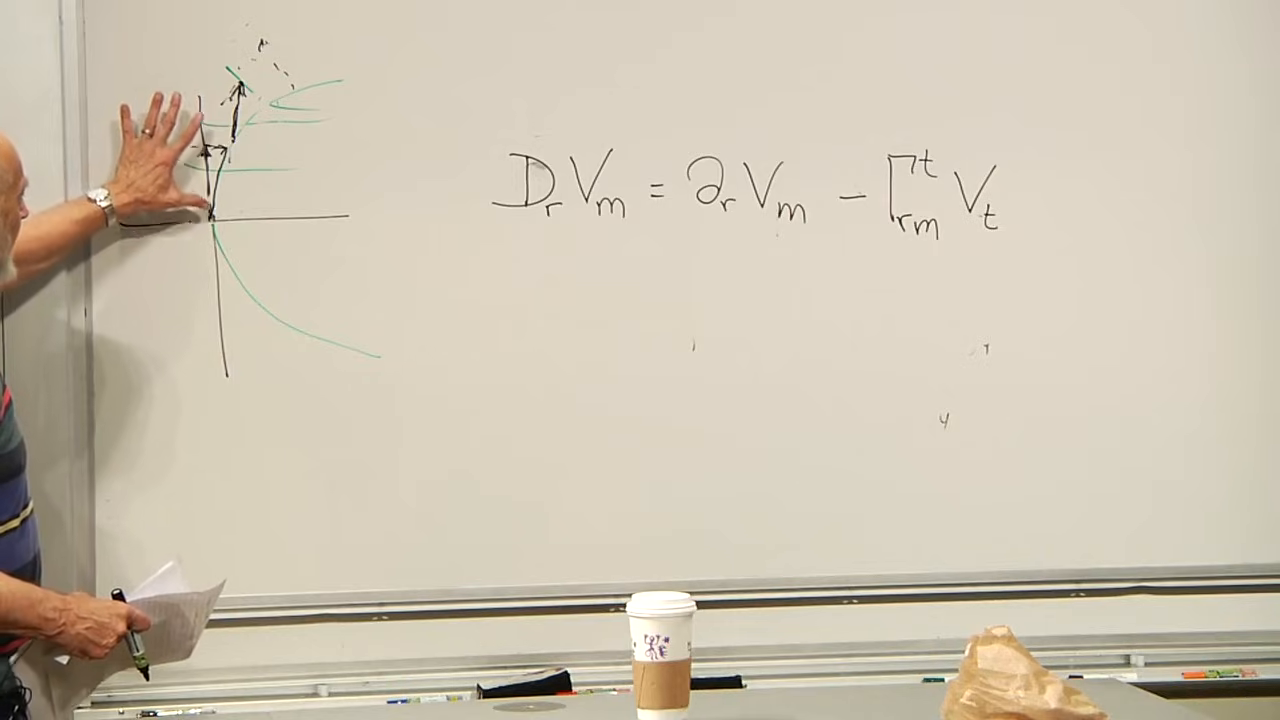
\includegraphics[width=\linewidth]{lecture_03_figure_12.png}
\caption{余ベクトルの共変微分：通常の成分変化から、動く基底によって引き起こされる変化を引いたもの。}
\lectureframe{00:49:50}
\end{figure}

\begin{classroomqa}
\audiencequestion{
\(\nabla_rV_m=\partial_rV_m-\Gamma^t{}_{rm}V_t\)は任意の座標で成り立つか、また正規座標では何になるか。}
\lecturerresponse{完全な式は任意の座標で成り立つ。正規座標の選ばれた点では、計量の一階微分、したがってクリストッフェル記号が消え、
\(\partial_rV_m\)だけが残る。その点から離れると、同じ正規座標チャートであっても一般には接続係数はゼロでない。
\lecturetimestamp{00:50:22}}
\end{classroomqa}

共変微分がそう名づけられているのは、対象全体\(\nabla_rV_m\)がテンソルとして共変的に変換するからであり、その名は単に下付き微分添字についての注釈ではない。クリストッフェル項は、偏微分の非テンソル的変換をまさに修復するものである。

\begin{figure}[H]
\centering
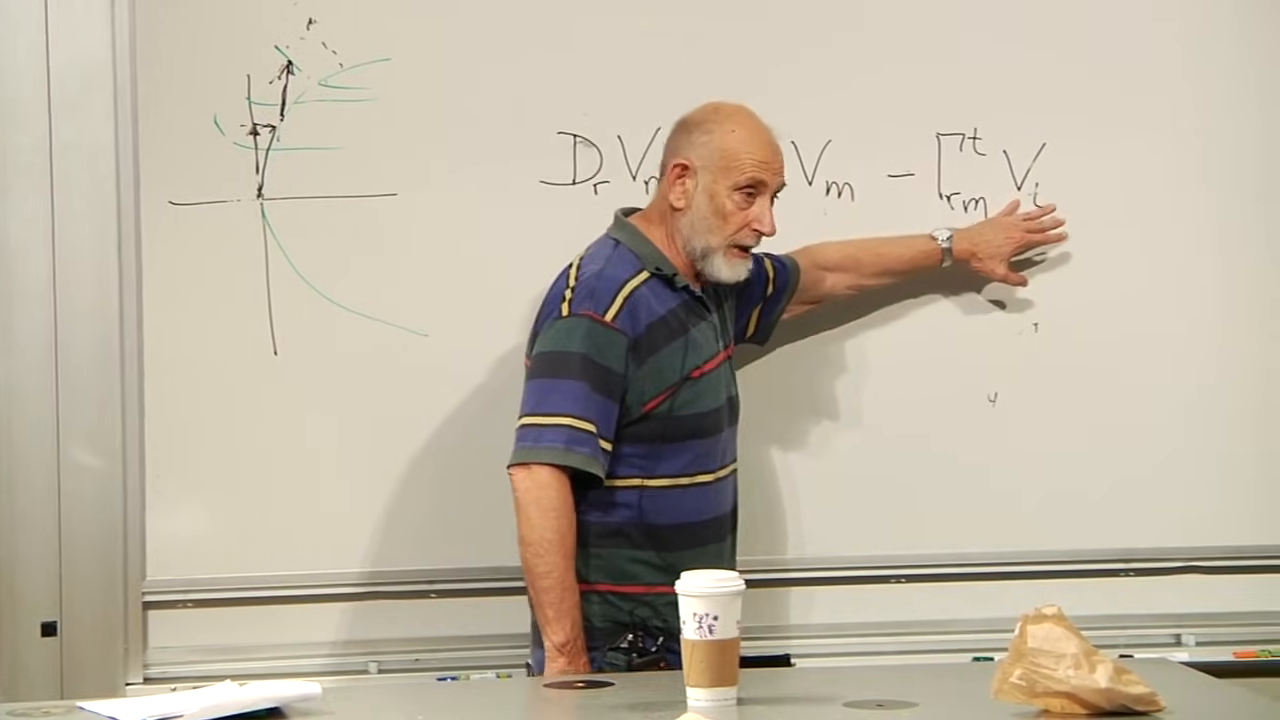
\includegraphics[width=\linewidth]{lecture_03_figure_13.png}
\caption{完全な余ベクトル微分とその接続補正。}
\lectureframe{00:51:30}
\end{figure}

\begin{classroomqa}
\audiencequestion{これは流体の流れで用いられる対流微分と関係があるか。}
\lecturerresponse{講義は慎重に、関係はあると答える。流体力学も、流れによって運ばれる変化と固定された座標点で見られる変化とを区別しており、曲がった座標や曲がった空間における流体方程式には共変微分が現れる。両演算子は定義上同一ではないが、どちらも記述とともに動く構造に対して素朴な微分を補正する。
\lecturetimestamp{00:52:31}}
\end{classroomqa}

ここで用いられている捩れのない接続では、
\begin{equation}
 \Gamma^t{}_{rm}=\Gamma^t{}_{mr}.
\label{eq:l3-torsion-free}
\end{equation}
より一般的な幾何学は捩れを持ちうるし、この対称性を必ずしも満たす必要はない。現在の接続は、一般相対性理論の標準的な計量定式化に関係するものである。

\begin{figure}[H]
\centering
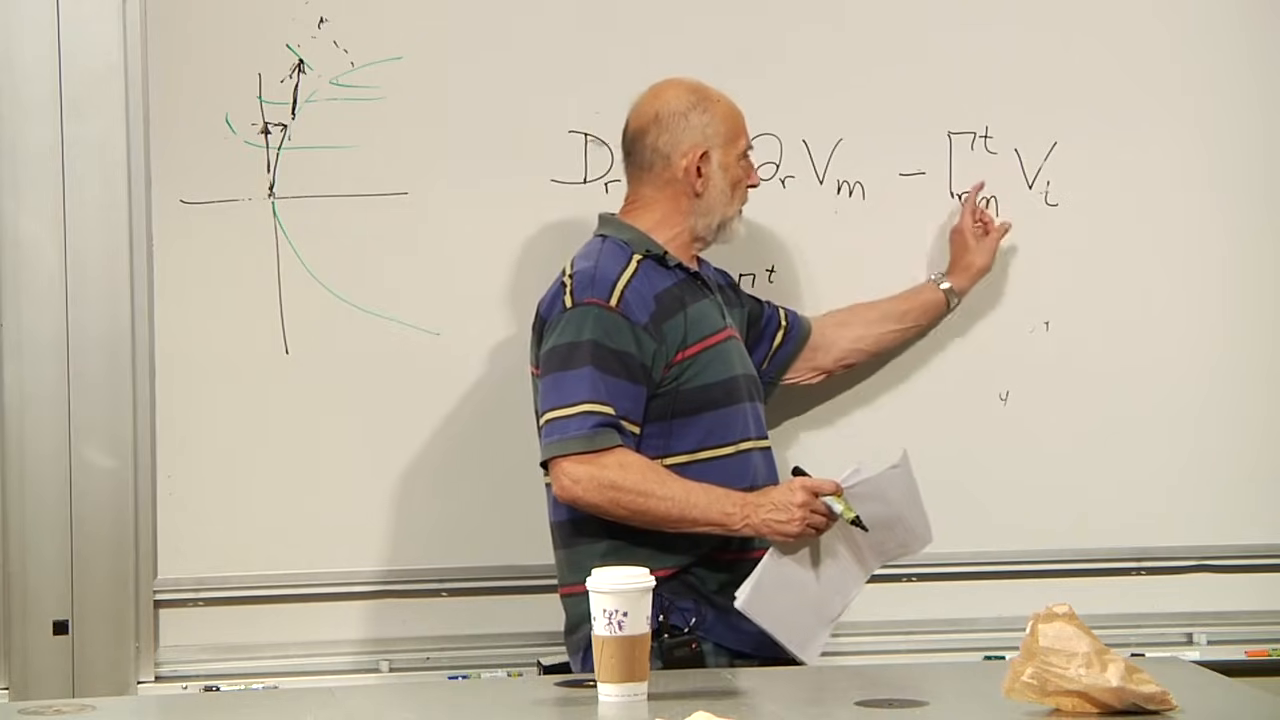
\includegraphics[width=\linewidth]{lecture_03_figure_14.png}
\caption{捩れのない幾何学の対称な接続係数として同定されたクリストッフェル記号。}
\lectureframe{00:54:30}
\end{figure}

有用な物理的類推がある。正規座標は一つの事象における自由落下系の役割を果たす。そこでは座標補正を消すことができる。任意の曲線座標は加速されたエレベーターに似ており、系自体が変化するために見かけの力が入り込む。この類推は局所的であり、単一の自由落下系が拡がった領域全体で重力を除去できない理由を、曲率が測ることになる。

\subsection{テンソルの各添字に一つずつの補正}

共変な二階テンソル\(T_{mn}\)では、各下付き添字がそれぞれ自身の接続補正を受ける：
\begin{equation}
 \nabla_sT_{mn}
 =\partial_sT_{mn}
 -\Gamma^t{}_{sm}T_{tn}
 -\Gamma^t{}_{sn}T_{mt}.
\label{eq:l3-rank-two-derivative}
\end{equation}
規則を覚えるには、一方の添字を観客として固定したまま他方を微分し、次に二番目の添字について繰り返せばよい。反変添字は反対符号の対応する項を受ける。

\begin{figure}[H]
\centering
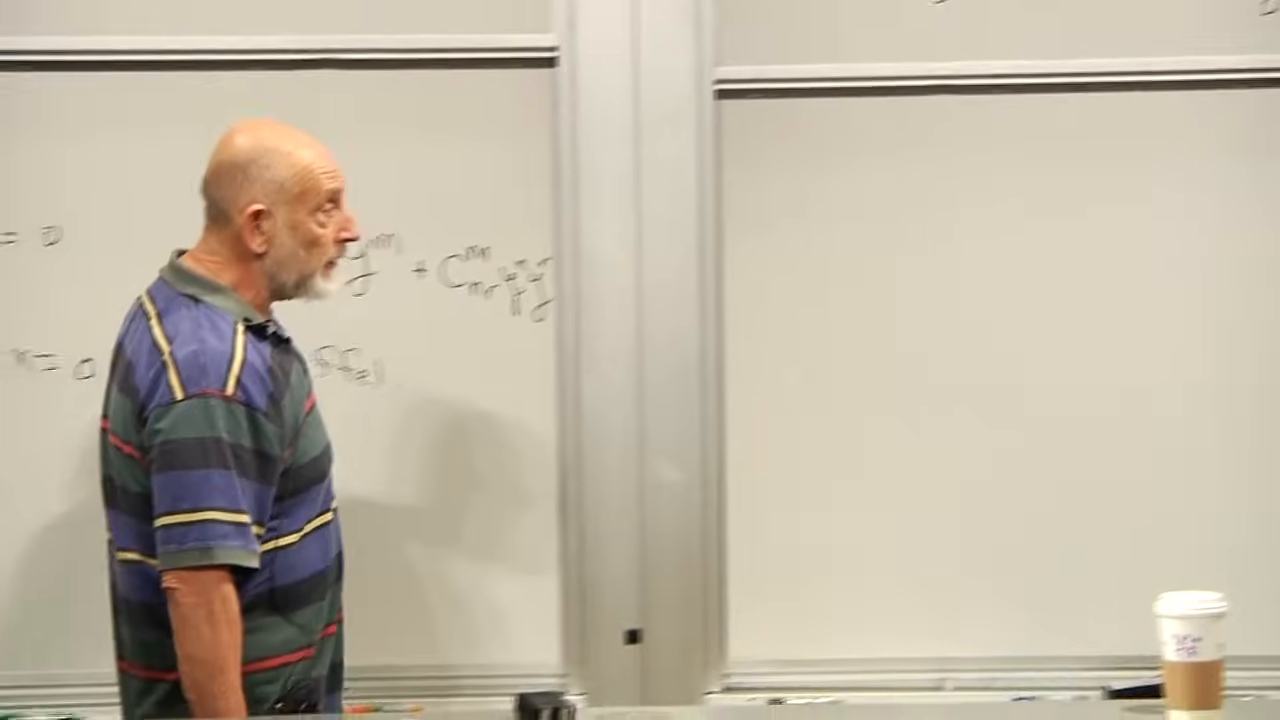
\includegraphics[width=\linewidth]{lecture_03_figure_15.png}
\caption{二階共変テンソルの共変微分であり、各下付き添字に一つずつのクリストッフェル補正がある。}
\lectureframe{01:01:50}
\end{figure}

\begin{classroomqa}
\audiencequestion{記号\(\partial_r\)自体は正規座標だけを指すのか、またテンソルの式はその系に制限されるのか。}
\lecturerresponse{いいえ。記法
\(\partial_r=\partial/\partial x^r\)は任意の座標系で意味を持ち、完全な共変微分の式は任意の座標に対して書かれる。クリストッフェル補正が消えるのは、正規系の選ばれた点においてのみである。\lecturetimestamp{00:57:22}}
\end{classroomqa}

\begin{classroomqa}
\audiencequestion{正規座標で共変微分が偏微分に帰着するとき、その帰着は選ばれた点においてのみか。クリストッフェル記号はテンソルか。}
\lecturerresponse{はい、帰着は点的である。クリストッフェル記号はテンソルではない。それらは正規座標において\(P\)で消え、別の座標系では同じ点でゼロでない値をとりうる。それらの非テンソル的変換こそが、\eqref{eq:l3-covector-derivative}における組み合わせがテンソルとして変換することを可能にする。
\lecturetimestamp{00:58:13}}
\end{classroomqa}

\begin{classroomqa}
\audiencequestion{共変微分は実際には何に使われるのか。}
\lecturerresponse{場の方程式にである。重力場は点ごとに変化するため、その方程式には微分が含まれなければならない。同時に、方程式はどの座標系でも同じ内容を持たなければならない。共変微分はテンソルをテンソルに変えるため、その真偽が特定の基準系に依存しない微分方程式を可能にする。\lecturetimestamp{01:02:35}}
\end{classroomqa}

\begin{classroomqa}
\audiencequestion{共変微分に座標微分を掛けることで、隣接する点の間の変化を記述できるか。}
\lecturerresponse{できる。無限小変位\(dx^s\)に沿った共変的な変化は\(dx^s\nabla_sT\)である。偏微分の項は成分の変化を測り、接続の項は座標基底の変化を担う。極座標における平坦空間でさえ、この区別が必要である。\lecturetimestamp{01:03:22}}
\end{classroomqa}

\section{計量整合性が接続を決定する}

2階の規則を計量に適用する。正規座標における\(P\)では、\(\partial_sg_{mn}=0\)かつ\(\Gamma^t{}_{sm}=0\)であるから、\(\nabla_sg_{mn}=0\)となる。共変微分はテンソルであるから、この点ごとの結果はどの座標系でも成り立つ：
\begin{equation}
 \nabla_sg_{mn}=0.
\label{eq:l3-metric-compatibility}
\end{equation}
これが計量整合性である。これは平行移動が計量を保ち、したがって長さと角度を保つことを述べている。

\begin{figure}[H]
\centering
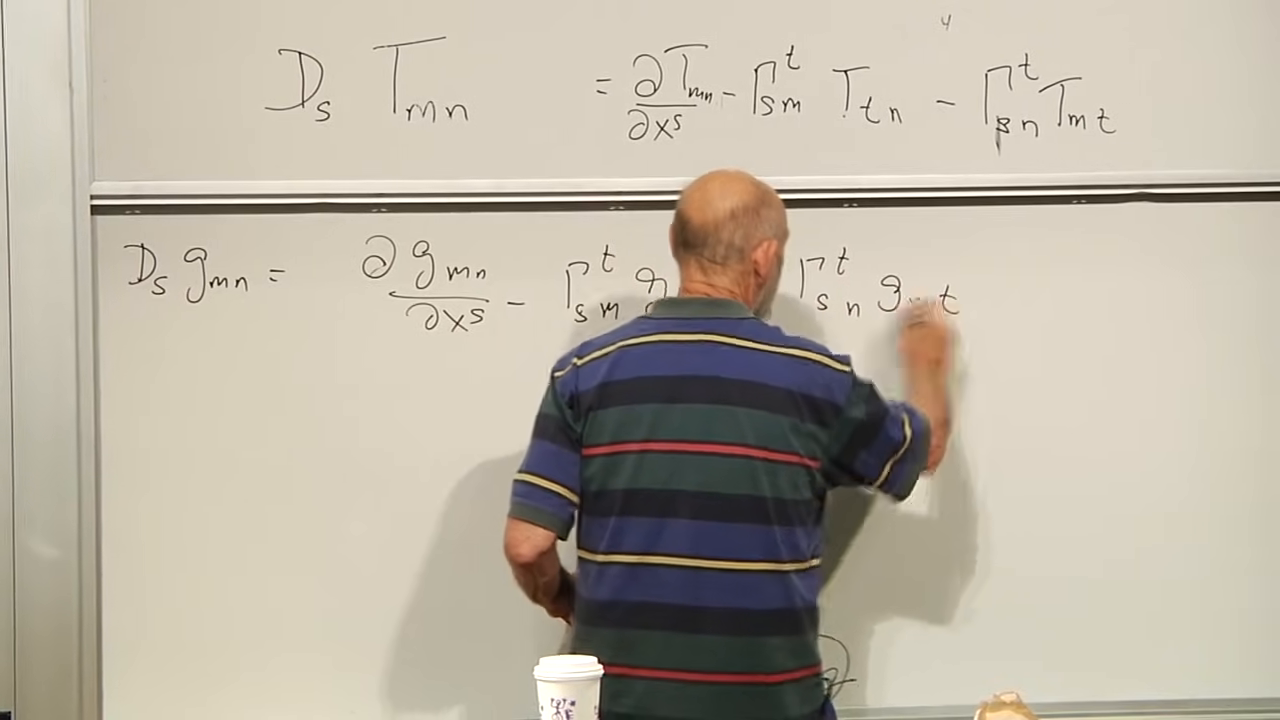
\includegraphics[width=\linewidth]{lecture_03_figure_16.png}
\caption{計量整合性の方程式は、計量から接続を導出する出発点となる。}
\lectureframe{01:06:20}
\end{figure}

\eqref{eq:l3-metric-compatibility}を展開すると
\begin{equation}
 0
 =\partial_sg_{mn}
 -\Gamma^t{}_{sm}g_{tn}
 -\Gamma^t{}_{sn}g_{mt}.
\label{eq:l3-compat-expanded}
\end{equation}
となる。微分と計量の添字を巡回的に置換したもう2つの式を書く：
\begin{align}
 0
 &=\partial_mg_{sn}
 -\Gamma^t{}_{ms}g_{tn}
 -\Gamma^t{}_{mn}g_{st},
\label{eq:l3-compat-m}\\
 0
 &=\partial_ng_{sm}
 -\Gamma^t{}_{ns}g_{tm}
 -\Gamma^t{}_{nm}g_{st}.
\label{eq:l3-compat-n}
\end{align}

\begin{figure}[H]
\centering
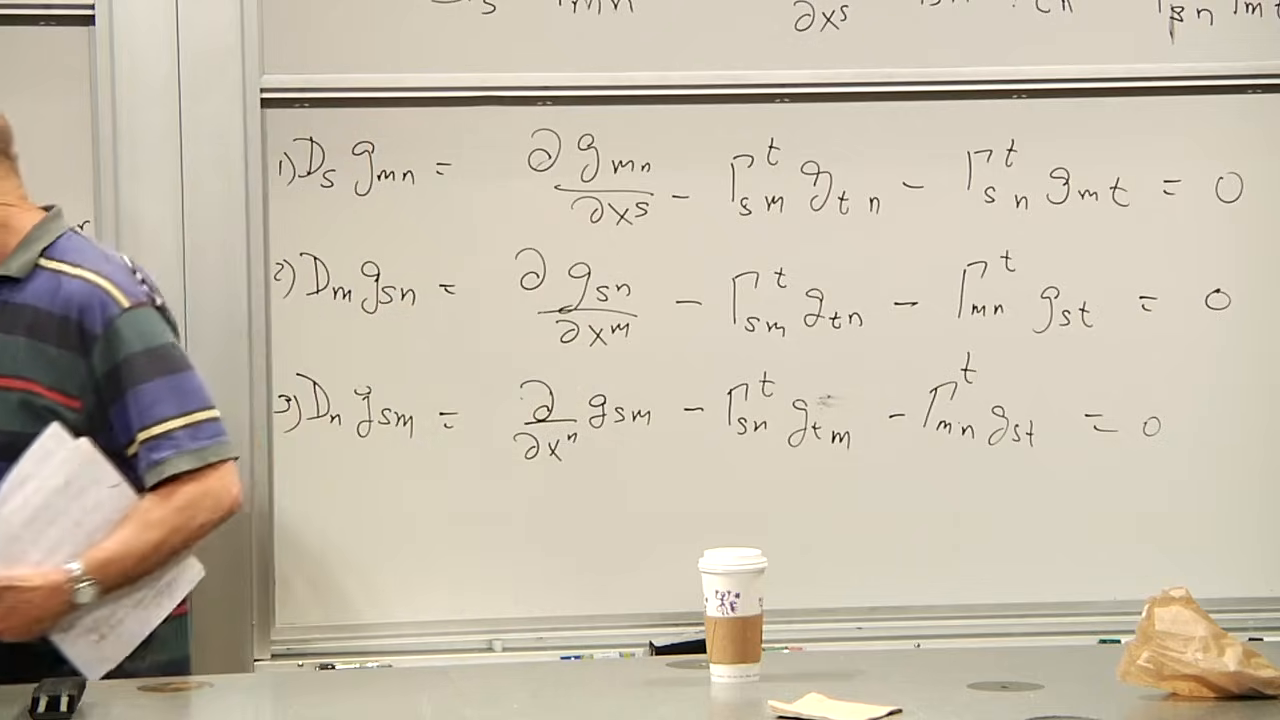
\includegraphics[width=\linewidth]{lecture_03_figure_17.png}
\caption{添字を置換した3つの計量整合性の方程式。}
\lectureframe{01:10:20}
\end{figure}

\eqref{eq:l3-compat-m}と\eqref{eq:l3-compat-n}を加え、次に\eqref{eq:l3-compat-expanded}を引く。捩れのない対称性\eqref{eq:l3-torsion-free}を用いると、不要な接続の項が相殺される：
\begin{equation}
 \partial_mg_{sn}+\partial_ng_{sm}-\partial_sg_{mn}
 =2\Gamma^t{}_{mn}g_{st}.
\label{eq:l3-isolate-gamma-lowered}
\end{equation}

\begin{figure}[H]
\centering
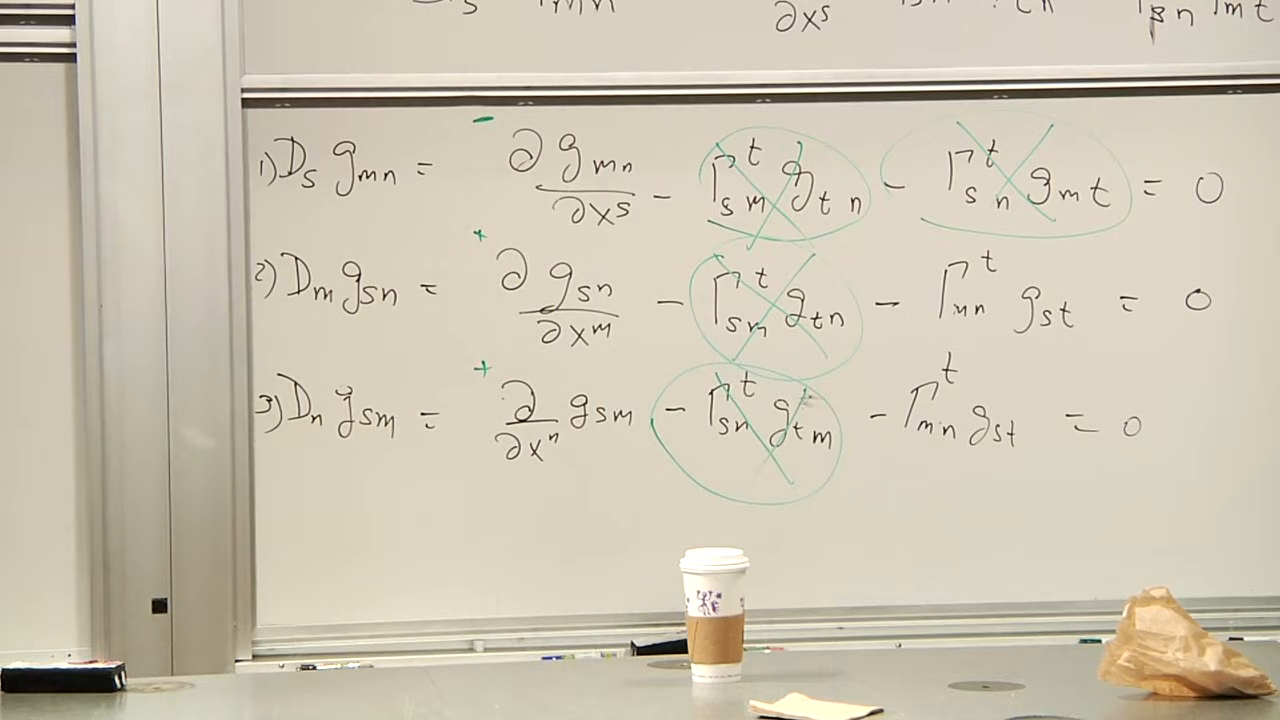
\includegraphics[width=\linewidth]{lecture_03_figure_18.png}
\caption{2つの整合性の方程式を加え、3番目を引くと、不要なクリストッフェル項が相殺される。}
\lectureframe{01:12:10}
\end{figure}

\(g^{rs}\)を掛けると接続が分離される：
\begin{equation}
 \boxed{
 \Gamma^r{}_{mn}
 =\frac12 g^{rs}
 \left(
 \partial_mg_{sn}
 +\partial_ng_{sm}
 -\partial_sg_{mn}
 \right)}
\label{eq:l3-christoffel}
\end{equation}
したがって、レヴィ・チヴィタ接続は計量とその1階微分から構成される。これが、クリストッフェル記号が正規座標の中心で消えると約束された理由である。

\begin{figure}[H]
\centering
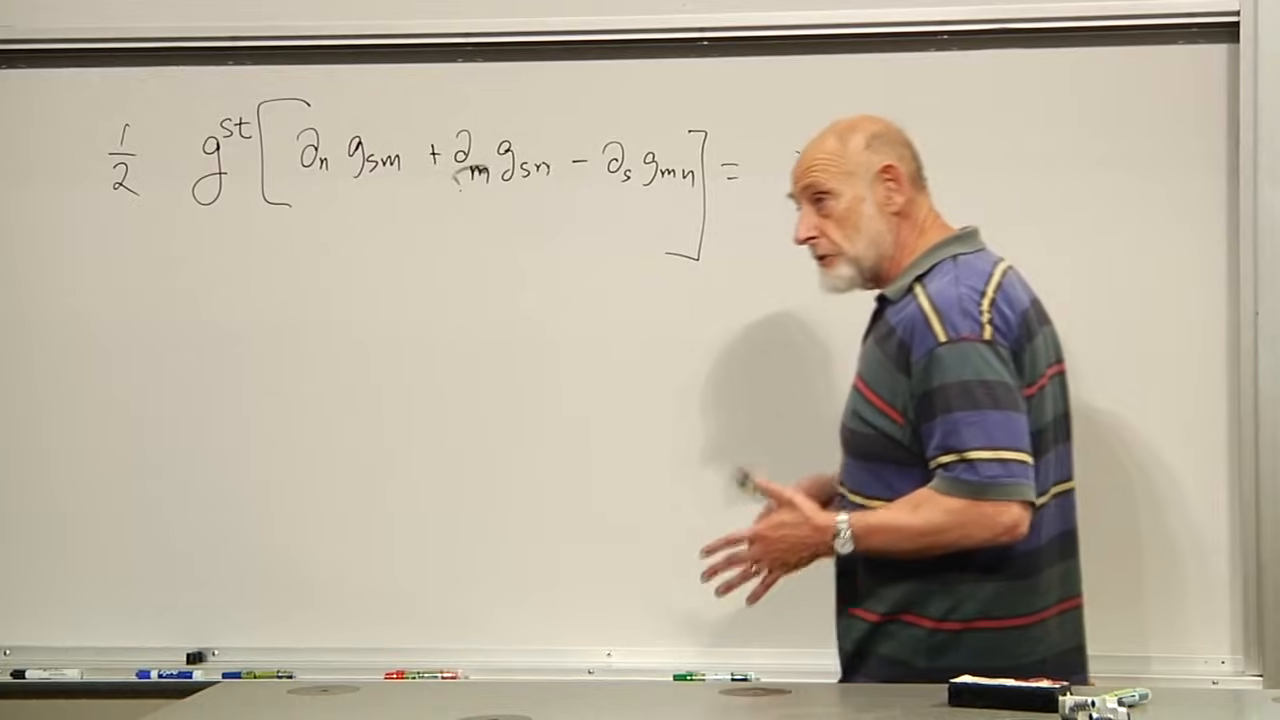
\includegraphics[width=\linewidth]{lecture_03_figure_19.png}
\caption{逆計量が、下付きの接続方程式からクリストッフェル記号を分離する。}
\lectureframe{01:16:10}
\end{figure}

\begin{classroomqa}
\audiencequestion{なぜ3つの計量整合性の方程式はすべてゼロに等しいとされたのか。}
\lecturerresponse{正規座標における選ばれた点では、計量の通常の微分が消え、クリストッフェル記号も消える。したがってそこでは計量の共変微分はゼロである。他の任意の点でこの主張を確立するには、その点を中心とする正規枠をとり、繰り返せばよい。\(\nabla_sg_{mn}\)はテンソルであるから、その消滅は座標に依存しない。\lecturetimestamp{01:14:27}}
\end{classroomqa}

\begin{classroomqa}
\audiencequestion{計量とクリストッフェル配列の次元は何であり、なぜ4次元では40個の独立なクリストッフェル成分が存在するのか。}
\lecturerresponse{\(d\)次元では、\(g_{mn}\)は対称な\(d\times d\)行列である。接続は3つの添字を持つ。各固定された上付き添字\(r\)に対し、対称な下付きの対\(mn\)は\(d(d+1)/2\)通りの選択を持つ。したがって捩れのない接続は\(d^2(d+1)/2\)個の独立な成分を持ち、\(d=4\)のとき40個である。\lecturetimestamp{01:16:18}}
\end{classroomqa}

\begin{figure}[H]
\centering
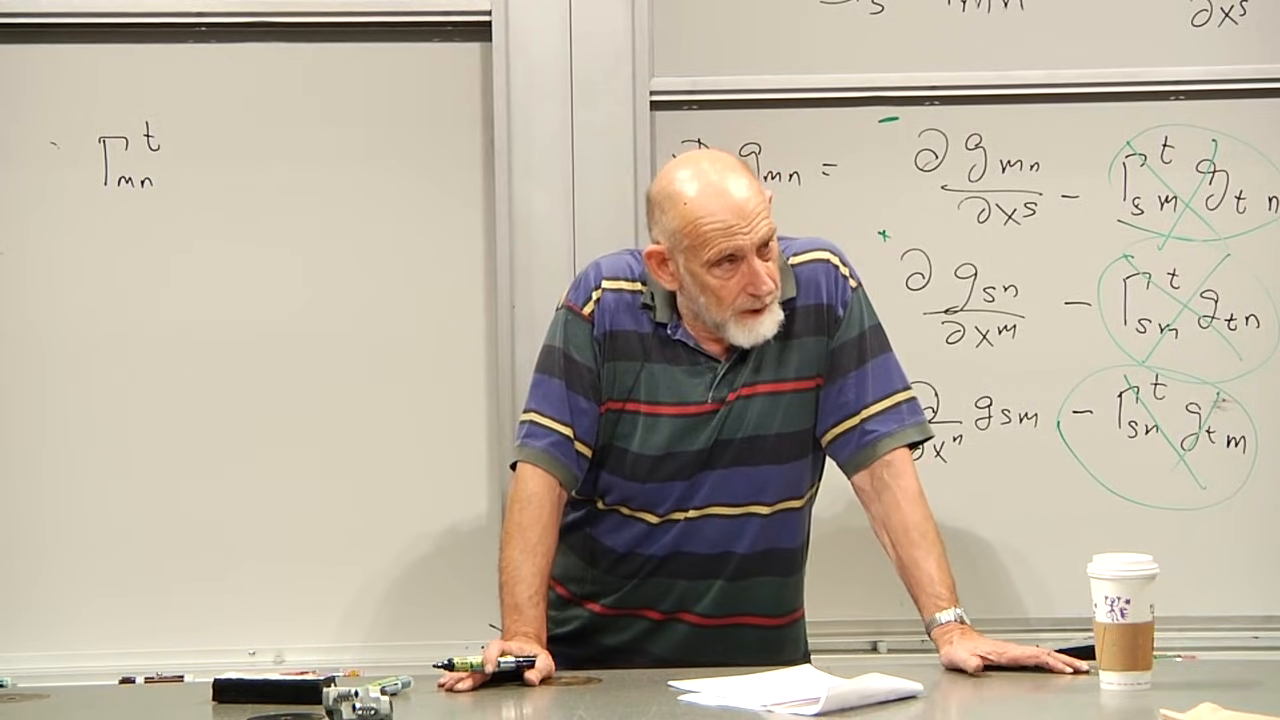
\includegraphics[width=\linewidth]{lecture_03_figure_20.png}
\caption{成分の数え方についての議論中の板書：対称な下付きの対に対して10通り、上付き添字に対して4通りの選択。}
\lectureframe{01:16:30}
\end{figure}

\begin{classroomqa}
\audiencequestion{\eqref{eq:l3-christoffel}にはどの計量が現れるのか。点ごとに異なる正規座標の計量を使わなければならないのか。}
\lecturerresponse{この公式は、計算のために選んだ任意の大域的または局所的な座標における計量の成分を用いる。正規座標は、この規則を導出するために用いられる局所的な道具にすぎない：ある点で正規枠に移り、そこで微分し、結果を変換して戻し、その後補助的な枠を捨てる。\eqref{eq:l3-christoffel}が分かれば、それは関心のある任意の座標で直接評価される。\lecturetimestamp{01:17:21}}
\end{classroomqa}

\begin{classroomqa}
\audiencequestion{\(\nabla_sg_{mn}=0\) またはクリストッフェルの公式は、その空間が平坦であることを教えてくれるのか。}
\lecturerresponse{いいえ。計量整合性は、曲がっていても平坦でも、すべてのレヴィ・チヴィタ接続に対して成り立つ。クリストッフェル記号は、極座標で書かれた平坦な平面においてさえ、ゼロでない値をとりうる。ある座標チャートのある領域全体で \(\Gamma^r{}_{mn}\) がすべて消えるなら、そのチャートはそこでデカルト座標であり、その領域は平坦である。しかし、それらが消えないことだけでは曲率を診断できない。\(\Gamma\) の微分と積から作られるテンソルが依然として必要である。\lecturetimestamp{01:19:27}}
\end{classroomqa}

\section{円錐は接続が明らかにできないものを明らかにする}

丸みを帯びた円錐を考える。その先端から離れたところでは、紙で作った通常の円錐で近似できる。平坦な円板から扇形を切り取り、露出した辺を貼り合わせる。残った紙はどこも引き伸ばされていない。局所的には、継ぎ目と先端から離れたすべての点は依然として平坦である。欠けている扇形は欠損角 \(\Delta\) によって記録される。

\begin{figure}[H]
\centering
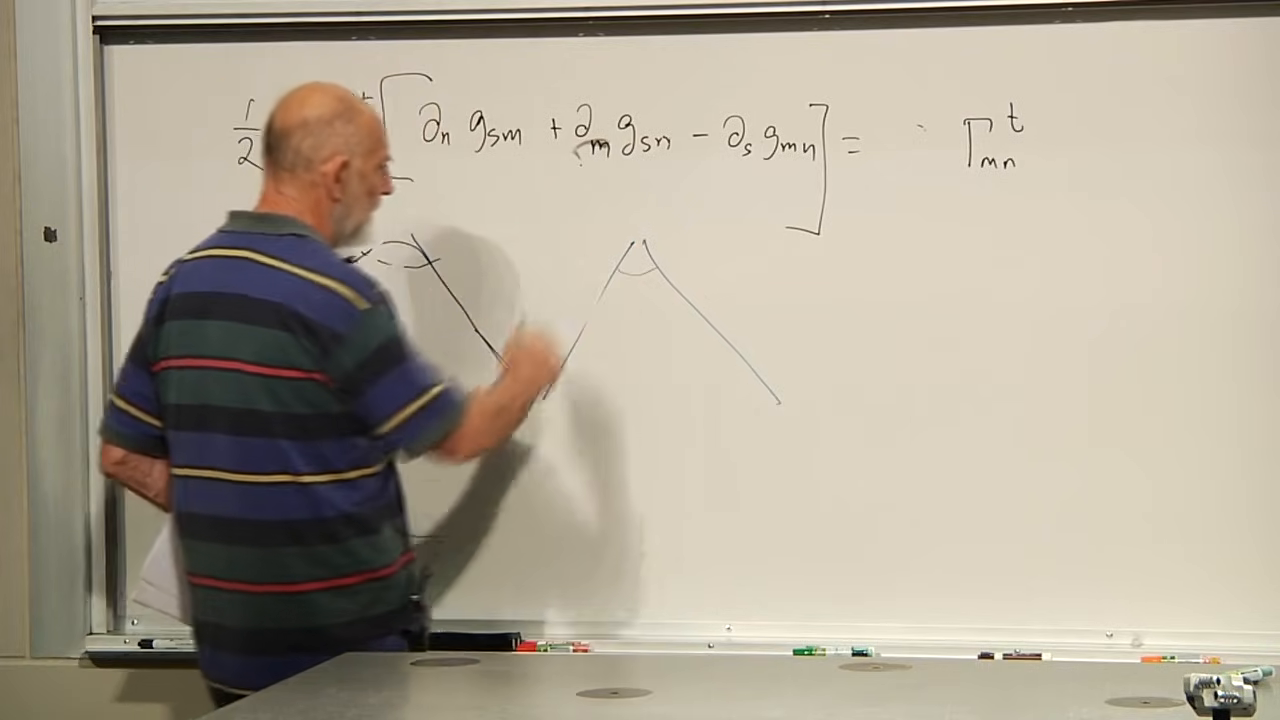
\includegraphics[width=\linewidth]{lecture_03_figure_21.png}
\caption{先端から離れたところでは局所的に平坦であるが、先端に非自明な曲率が集中している幾何学として導入される円錐。}
\lectureframe{01:23:00}
\end{figure}

\begin{figure}[H]
\centering
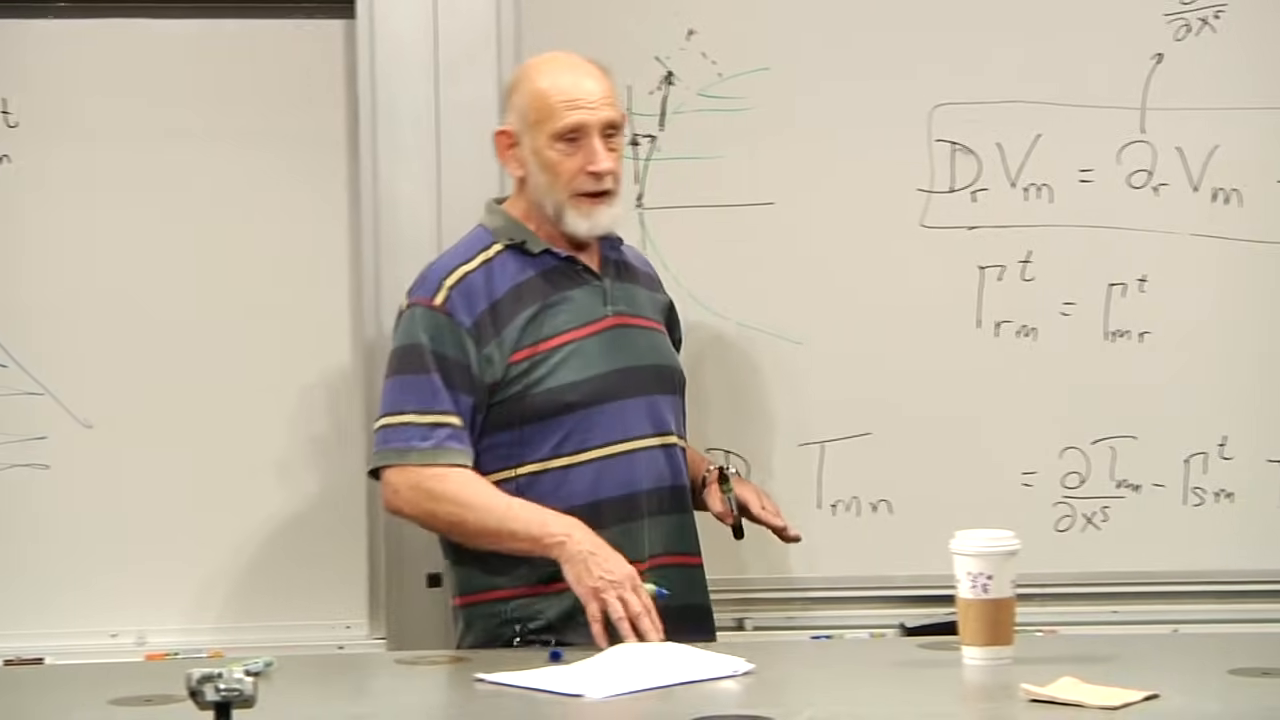
\includegraphics[width=\linewidth]{lecture_03_figure_22.png}
\caption{円板から扇形を切り取り、その辺を同一視すると、円錐欠損角が生じる。}
\lectureframe{01:24:20}
\end{figure}

紙による構成は、この区別を具体的にする。切り取った紙の上で、通常の平面において平行を保ちながらベクトルを輸送する。扇形の辺を同一視した後、先端を一周する経路は、輸送されたベクトルが初期の向きに対して回転して、出発点に戻る。

\begin{figure}[H]
\centering
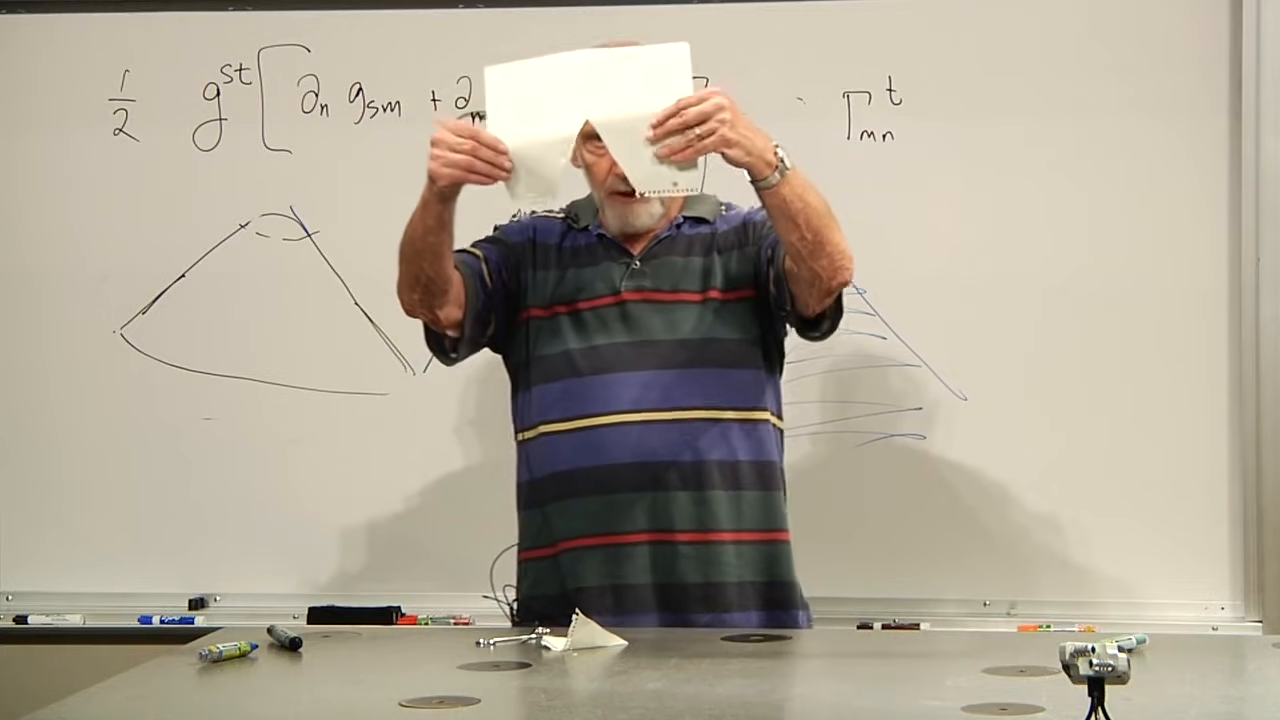
\includegraphics[width=0.78\linewidth]{lecture_03_figure_23.png}
\caption{紙の円錐の実演：扇形を取り除いた平坦な紙は、切り口の辺を接合すると円錐になる。}
\lectureframe{01:25:10}
\end{figure}

\begin{figure}[H]
\centering
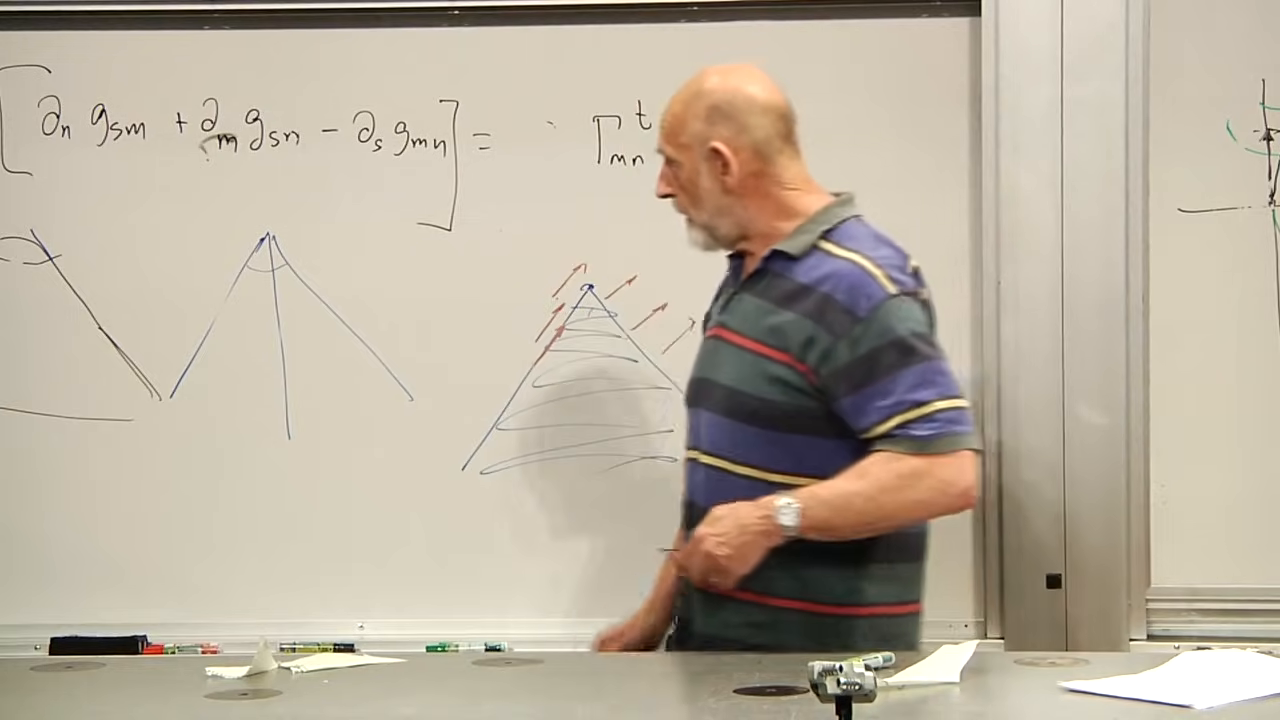
\includegraphics[width=\linewidth]{lecture_03_figure_24.png}
\caption{辺を同一視する前に、切り取った扇形の上に描かれたベクトル。}
\lectureframe{01:27:40}
\end{figure}

この回転はホロノミーである。それは一つの線分に沿った座標のまずい選択によって引き起こされるのではない。各々の小さな線分は局所的に平坦な枠で扱うことができる。この効果は、それらの局所的な比較を閉じたループの周りで合成した後に初めて現れる。理想的な円錐では、正味の回転は向きを除いて欠損角に等しい。

\begin{figure}[H]
\centering
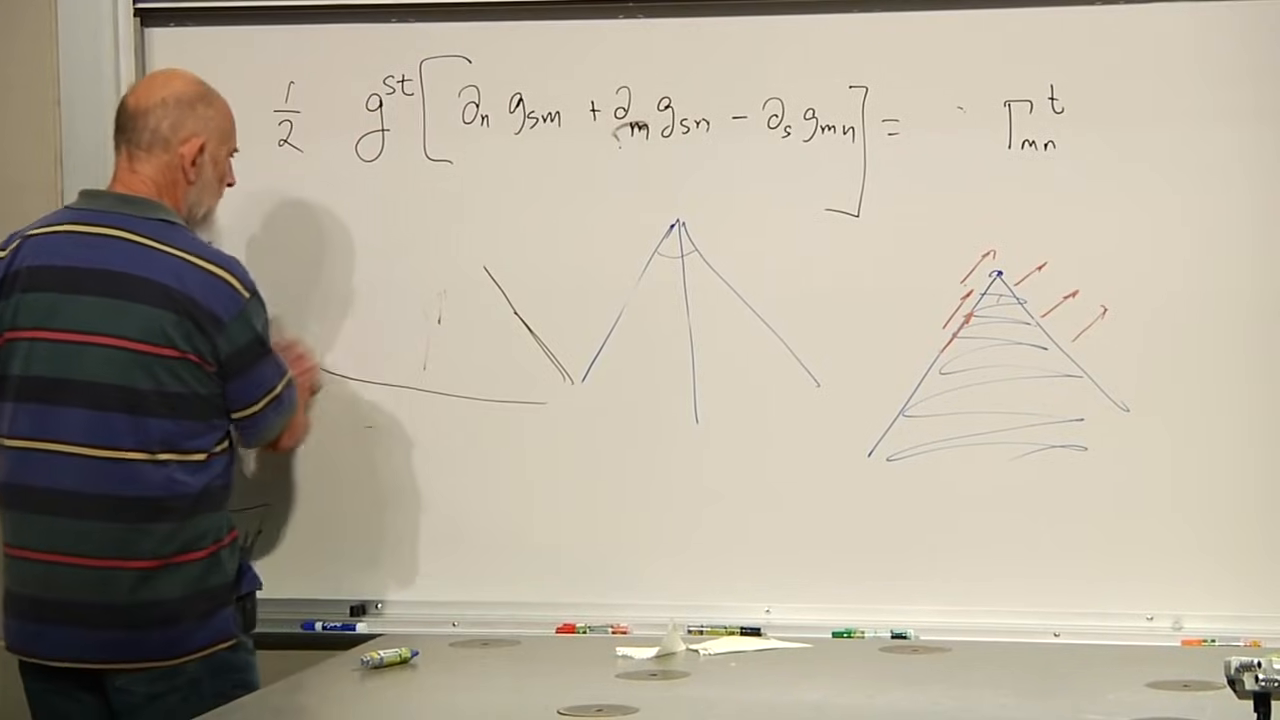
\includegraphics[width=\linewidth]{lecture_03_figure_25.png}
\caption{円錐の先端の周りの平行輸送は、向きが回転したベクトルを返す。ホロノミーは囲まれた曲率を記録する。}
\lectureframe{01:29:10}
\end{figure}

\section{無限小ループを巡る二つの経路}

有限のループを微小な座標長方形に置き換える。一つの角から出発し、まず \(r\) 方向に、次に \(s\) 方向に輸送する。その結果を、まず \(s\) 方向に、次に \(r\) 方向に輸送した結果と比較する。平坦なデカルト座標では二つの経路は一致する。曲がった幾何学では、一般には一致しない。

\begin{figure}[H]
\centering
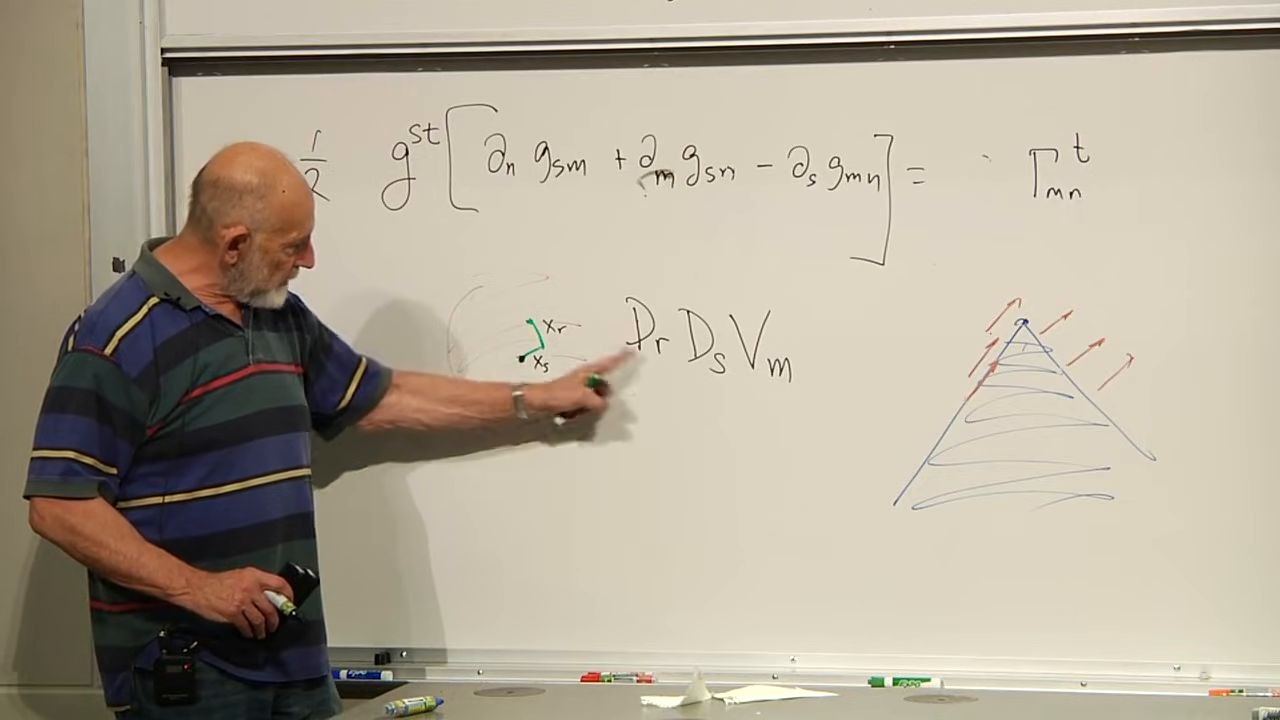
\includegraphics[width=\linewidth]{lecture_03_figure_26.png}
\caption{座標長方形の周りの無限小輸送の二つの順序。}
\lectureframe{01:31:40}
\end{figure}

代数的な尺度は共変微分の交換子である：
\begin{equation}
 \left(\nabla_s\nabla_r-\nabla_r\nabla_s\right)V_n.
\label{eq:l3-commutator}
\end{equation}
通常の混合偏微分は滑らかな関数上で交換する。ここでの不一致は、ベクトル成分だけでなく接続項も微分することから生じる。

\begin{figure}[H]
\centering
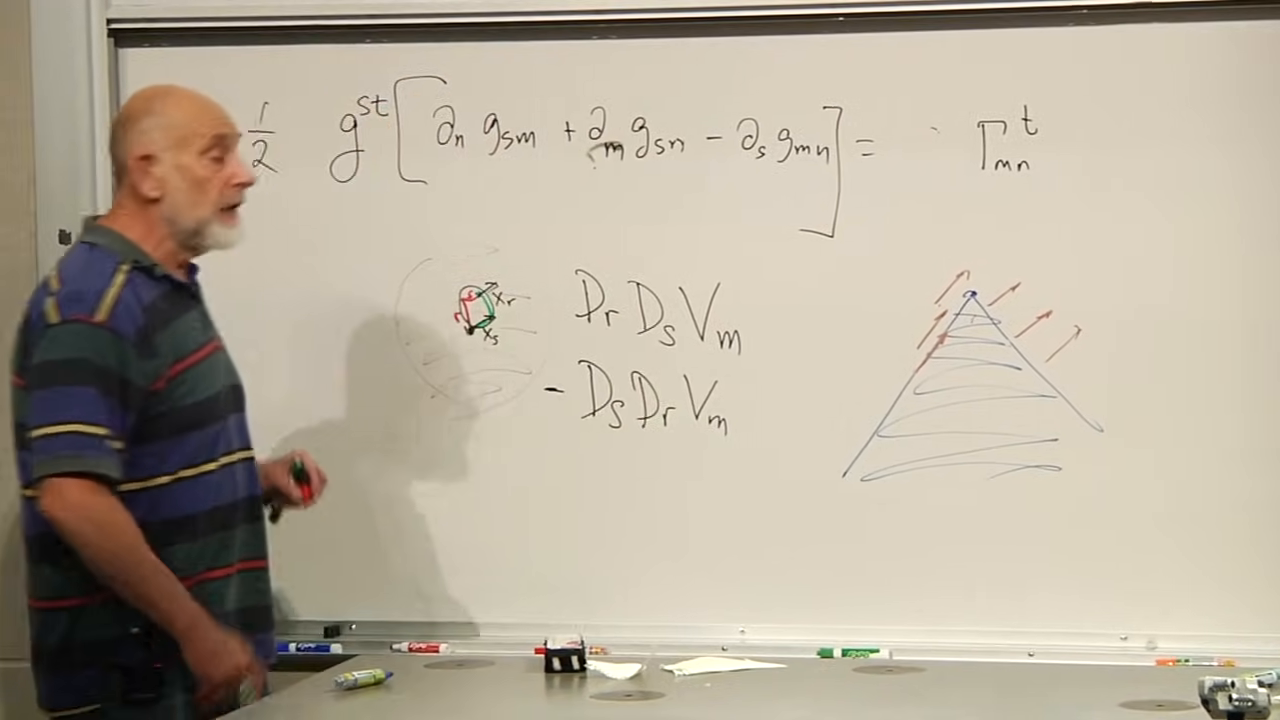
\includegraphics[width=\linewidth]{lecture_03_figure_27.png}
\caption{共変微分の二つの順序の差によって表される無限小ループ。}
\lectureframe{01:33:20}
\end{figure}

それを計算するには、まず
\[
 T_{rn}=\nabla_rV_n
\]
を二階の共変テンソルとみなす。次に
\eqref{eq:l3-rank-two-derivative} を用いて \(T_{rn}\) を
\(s\) 方向に微分する。\(r\) と \(s\) を入れ替えて繰り返し、引き算する。この操作は長いが機械的である：展開し、積の法則を適用し、\(V_n\) の二階偏微分を含む項を相殺する。

\begin{figure}[H]
\centering
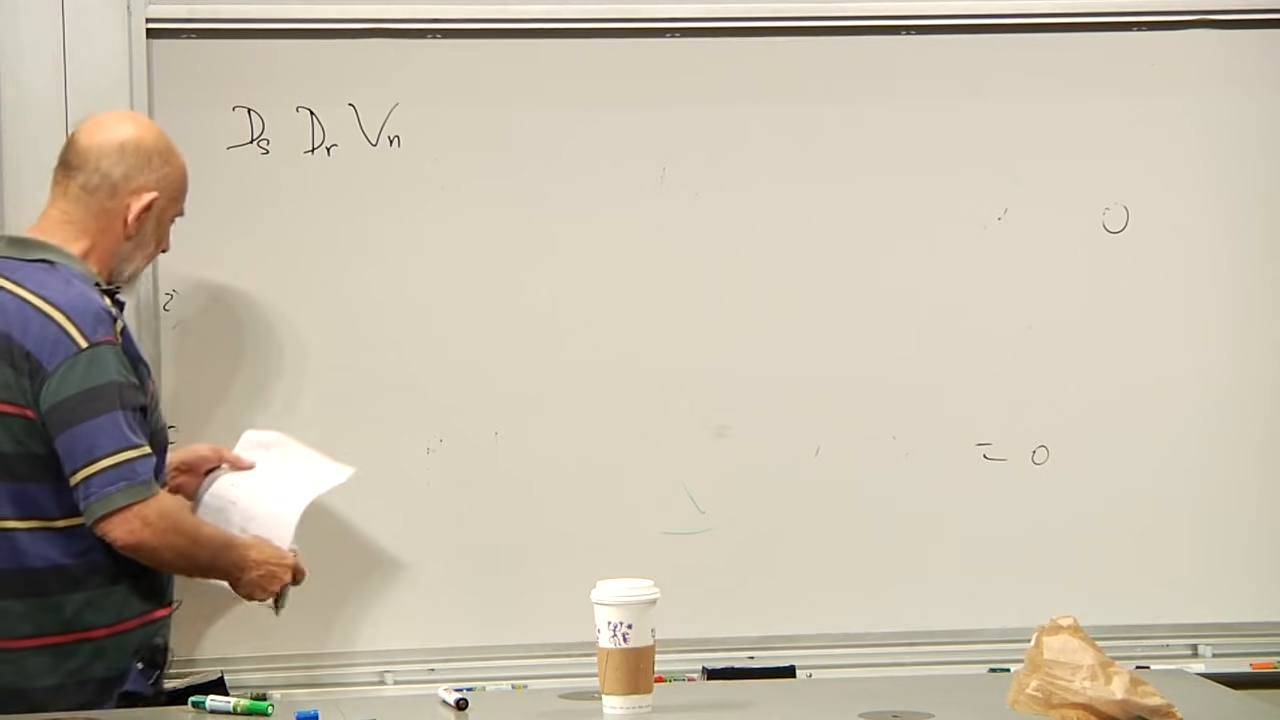
\includegraphics[width=\linewidth]{lecture_03_figure_28.png}
\caption{\(\nabla_rV_n\) を二階のテンソルとして扱うことから二重共変微分を始める。}
\lectureframe{01:35:40}
\end{figure}

黒板で採用した規約を用いると、結果は
\begin{equation}
 \left(\nabla_s\nabla_r-\nabla_r\nabla_s\right)V_n
 =R_{srn}{}^tV_t.
\label{eq:l3-riemann-commutator}
\end{equation}

\begin{figure}[H]
\centering
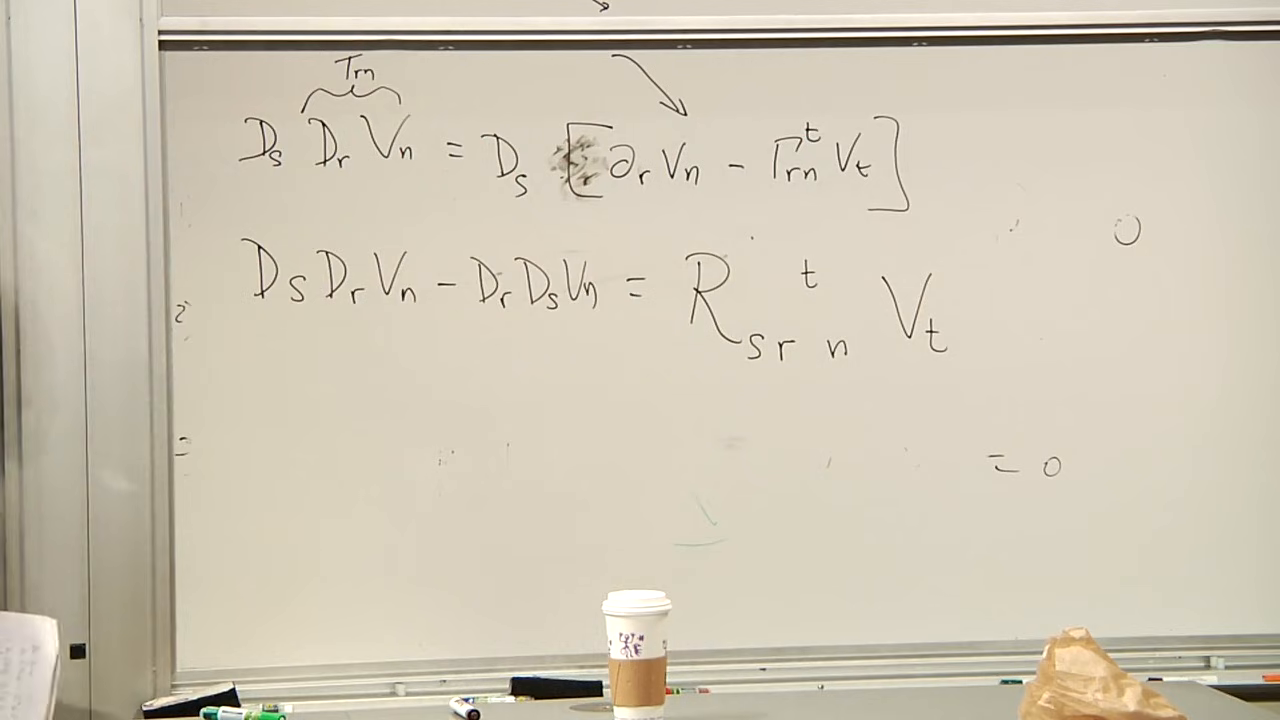
\includegraphics[width=\linewidth]{lecture_03_figure_29.png}
\caption{共変微分の交換子は、曲率テンソルの余ベクトルへの作用を定義する。}
\lectureframe{01:38:30}
\end{figure}

この交換子の順序に対して、
\begin{equation}
\begin{split}
 R_{srn}{}^t
={}&
 \partial_r\Gamma^t{}_{sn}
 -\partial_s\Gamma^t{}_{rn}\\
&+\Gamma^p{}_{sn}\Gamma^t{}_{pr}
 -\Gamma^p{}_{rn}\Gamma^t{}_{ps}.
\end{split}
\label{eq:l3-riemann}
\end{equation}
他の教科書では符号を逆にしたり、添字を異なるように並べたりするかもしれない。規約は \eqref{eq:l3-riemann-commutator} と \eqref{eq:l3-riemann} の両方を書くことによって固定される。

\begin{figure}[H]
\centering
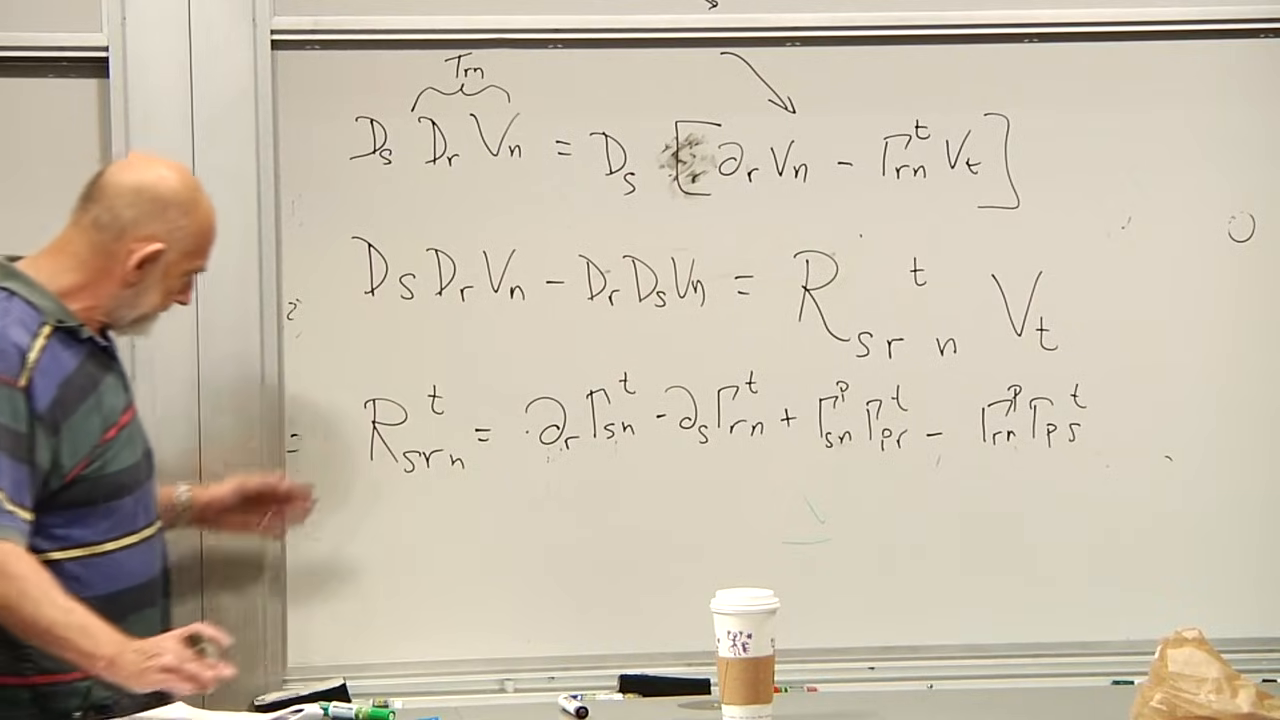
\includegraphics[width=\linewidth]{lecture_03_figure_30.png}
\caption{リーマンテンソル：接続の二つの微分と二つの二次の接続項。}
\lectureframe{01:39:40}
\end{figure}

式\eqref{eq:l3-christoffel}は、曲率が計量について二次で初めて現れる理由を示している。各\(\Gamma\)は\(g\)の一階導関数を含む。したがって、\eqref{eq:l3-riemann}の導関数項は\(g\)の二階導関数を含み、二次の項は一階導関数の積を含む。\(P\)における正規座標では、接続自体は消えるが、その導関数は一般には消えないため、曲率は生き残る：
\[
\begin{aligned}
 \Gamma^t{}_{mn}(P)&=0,\\
 R_{srn}{}^t(P)
 &=\partial_r\Gamma^t{}_{sn}(P)
 -\partial_s\Gamma^t{}_{rn}(P).
\end{aligned}
\]
導関数の階数を正しく保つことが重要である。リーマンテンソルは\(\Gamma\)の一階導関数を用いるが、これは計量について二次である。

これが求める診断法である。リーマンテンソルのすべての成分がある領域全体で消えるなら、その領域は局所的に平坦である。ある点でいずれかの成分が非零なら、座標のどのような変更によってもそこで曲率を除去することはできない。計算機代数システムは解析的な計量からこれらの成分を検査できるが、概念としては、平行移動が微小ループの周りで閉じないことにほかならない。

\section{潮汐重力としての曲率}

この幾何学的診断法には直接的な物理的意味がある。連結された三角形からなる柔軟な物体を想像しよう。平坦な領域では、それは応力なしに動かすことができる。内在的計量が曲がっている領域へそれを押し込むと、連結部の異なる部分がすべてその好ましい間隔と角度を保つことはできない。物体は伸びるか、縮むか、ずれるかを余儀なくされる。

\begin{figure}[H]
\centering
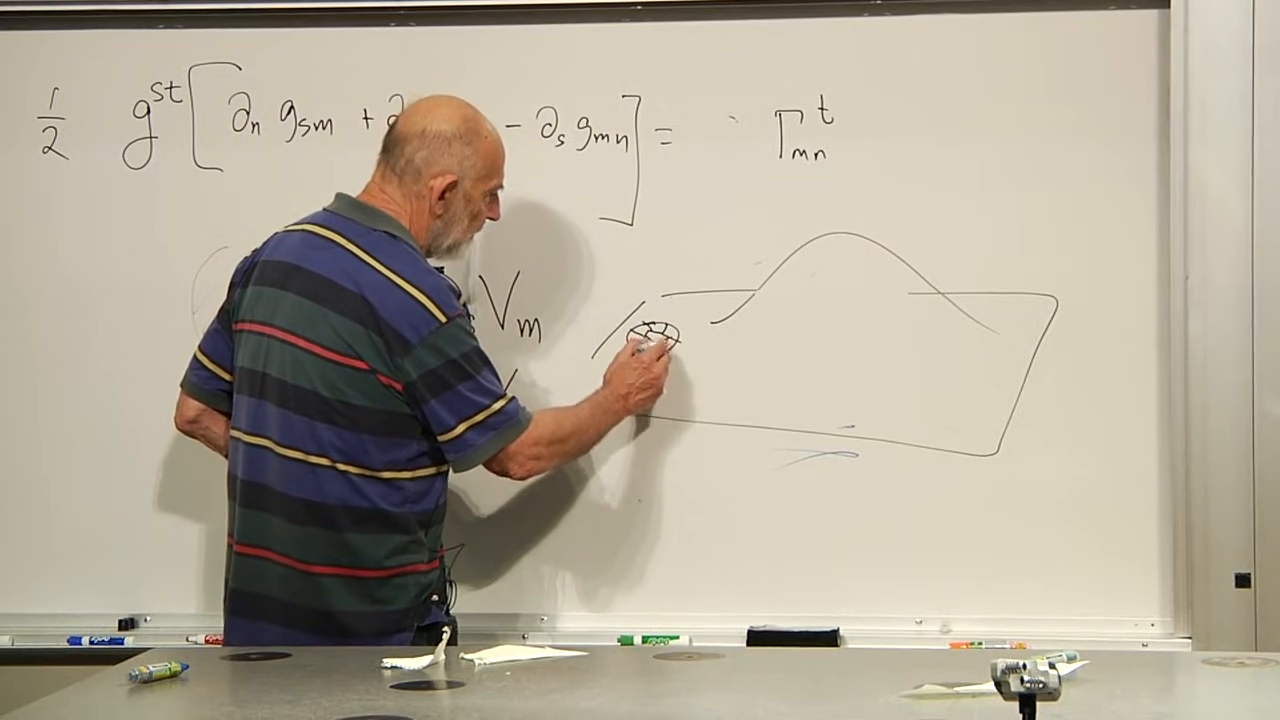
\includegraphics[width=\linewidth]{lecture_03_figure_31.png}
\caption{平坦な領域から曲がった膨らみへ動かされた連結物体は、局所計量に従うために変形しなければならない。}
\lectureframe{01:44:10}
\end{figure}

その変形は潮汐力の幾何学的対応物である。重力場では、隣り合う自由落下粒子は互いに対して加速しうる。ある方向は引き伸ばされ、別の方向は圧縮されるかもしれない。リーマンテンソルがこの相対加速度を支配する。後に測地線偏差として導入される言葉では、接ベクトル\(u^\mu\)と分離\(\xi^\mu\)に対して、
\begin{equation}
 \frac{D^2\xi^\mu}{D\tau^2}
 =-R^\mu{}_{\nu\rho\sigma}
 u^\nu\xi^\rho u^\sigma,
\label{eq:l3-geodesic-deviation-preview}
\end{equation}
であり、全体の符号は選ばれた曲率の規約に従う。この方程式はここでは導出されないが、曲率と潮汐応力が文字通り同じ局所物理であるという講義の主張を精密にするものである。

理想的な完全一様重力場には潮汐変化がなく、一様加速系へ移ることによって局所的に除去できる。孤立した質量がつくる実際の場は完全には一様でない。地球の場はほぼ動径方向を向き、位置とともに変化するので、隣り合う自由落下軌道は収束または発散する。

\begin{figure}[H]
\centering
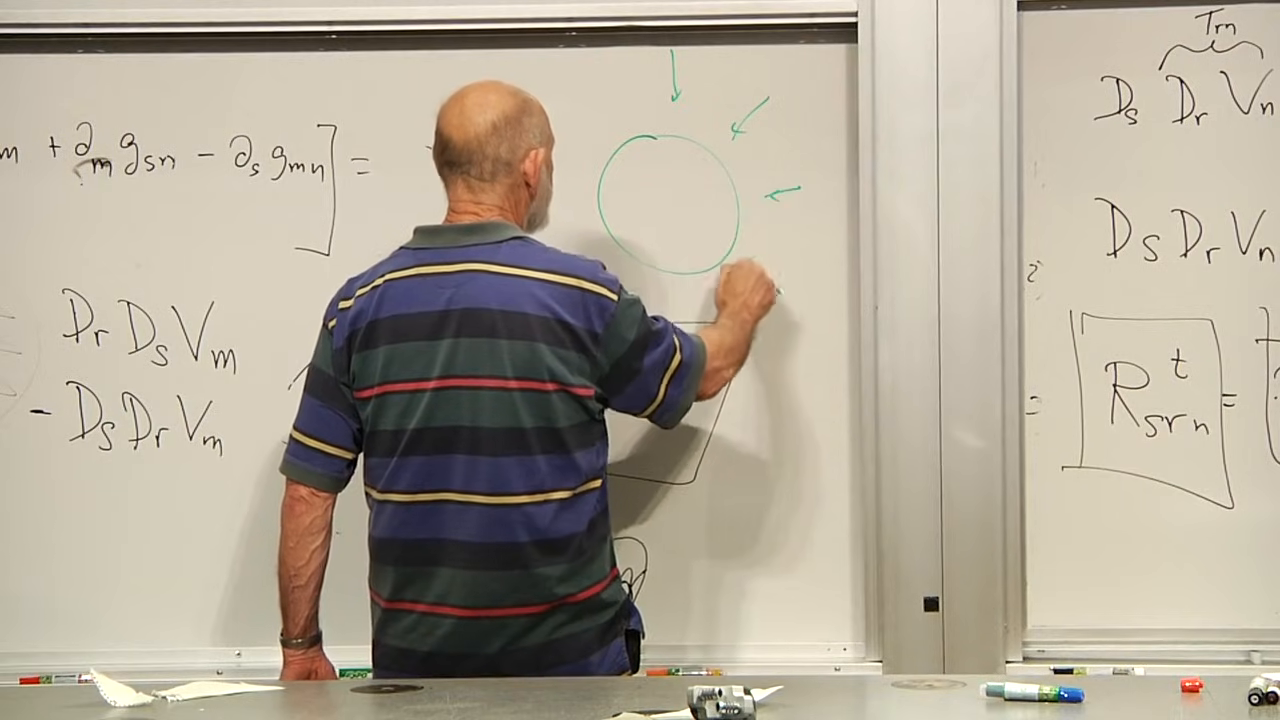
\includegraphics[width=\linewidth]{lecture_03_figure_32.png}
\caption{動径方向の重力場は拡がった物体にわたって変化し、潮汐重力として同定される相対加速度を生じる。}
\lectureframe{01:48:40}
\end{figure}

\begin{classroomqa}
\audiencequestion{真の重力場を、加速系で見られる見かけの場と区別するものは何か。}
\lecturerresponse{一様加速系は局所実験に対して一様重力場を模倣できるが、潮汐的な相対加速度を生じない。実在の物質がつくる場は場所ごとに変化するので、潮汐力を生じる。それらの力は、効果が単なる座標変換ではないことの不変な証拠である。完全に一様な実在の場は理想化であり、大きな物体の表面の十分小さな一部分の近くでは、実際の場は近似的にしか一様でありえない。\lecturetimestamp{01:46:54}}
\end{classroomqa}

\begin{classroomqa}
\audiencequestion{なぜ落下物体の大きさが潮汐効果にとって重要になるのか。}
\lecturerresponse{曲率は隣り合う位置を比較する。場が変化する長さスケールよりずっと小さい物体は、そのすべての部分でほとんど同じ加速度をサンプルし、ほとんど変形しない。拡がった物体はより大きな差をサンプルする。地球近傍で自由落下する細菌は無視できる潮汐応力を感じるだけであるが、講義の想像上の二千マイルの人ならひどく歪められるであろう。曲率は局所的な値をもつが、蓄積された変形は比較される分離に比例して大きくなる。
\lecturetimestamp{01:49:01}}
\end{classroomqa}

\begin{classroomqa}
\audiencequestion{平坦性がすべての点で曲率を調べることを要求するなら、そのテストは依然として無限の問題なのか。}
\lecturerresponse{解析的に与えられた計量に対しては、導関数と曲率成分は解析的表現である。それらを位置の関数として一度計算すれば、それらが恒等的に消えるかどうかをしばしば見て取ることができる。計量が数値表としてのみ与えられるなら、サンプルされた領域全体で曲率を推定し検査しなければならず、それは確かに高くつきうる。それでもなお、これはすべての点ですべての可能な座標系を探すよりはるかに明確に定義されている。
\lecturetimestamp{01:50:37}}
\end{classroomqa}

\section{確立されたこと}

この議論は今や一続きの連鎖として読むことができる：
\begin{enumerate}
 \item 任意に選んだ点において、座標は
 \(g_{mn}=\delta_{mn}\) および \(\partial_rg_{mn}=0\) とすることができる。
 \item テンソル成分の通常の導関数は、座標基底が点ごとに変化するため、テンソルとして変換されない。
 \item 接続はその基底の変化を補正し、共変微分を定義する。
 \item 計量整合性と捩率ゼロが、計量から接続を一意に決定する。
 \item 二つの共変微分はリーマンテンソルによって可換でない。その非可換性はホロノミー、計量の二次変分、潮汐重力を測る。
\end{enumerate}

したがって、約束された曲率の診断法は、特権的な大域座標系を選ぶことなく構成された。次の段階は、正定値リーマン幾何学からローレンツ時空へ移行し、これらの道具を恒星やブラックホールのシュヴァルツシルト幾何学に適用し、この講義の最後で保留にした測地線に戻ることである。